\documentclass{article}
\usepackage[utf8]{inputenc}
\usepackage[T1]{fontenc}
\usepackage[a4paper, portrait, margin=1in]{geometry}
\usepackage{graphicx}
\usepackage{subcaption}
\usepackage{xcolor}
\usepackage{colortbl}
\usepackage{amscd,amsmath,amssymb,amsthm}
\usepackage{array}
\usepackage{mathtools, mathbbol}
\usepackage{bbm,dsfont}
\usepackage{lipsum}
\usepackage{cancel}
\allowdisplaybreaks
\DeclareMathAlphabet{\mathbbold}{U}{bbold}{m}{n}
\parindent=15pt
\parskip=0pt plus 2pt

\newtheorem{theorem}{Theorem}
\newtheorem{lemma}{Lemma}

\newcommand{\0}{\mathbbold{0}}
\newcommand{\1}{\mathds{1}}
\newcommand{\2}{\mathbbold{2}}
\newcommand{\V}{\mathbb{V}}
\newcommand{\Dnk}{\mathbb{D}_{n \times k}}
\newcommand{\T}{^{\operatorname{T}}}
\newcommand{\diag}[1]{\text{diag}\!\left(#1\right)}
\newcommand{\Diag}[1]{\text{Diag}\!\left(#1\right)}
\newcommand{\Beta}[2]{\text{Beta}\!\left(#1,#2\right)}
\newcommand{\BBeta}[2]{\textbf{Beta}\!\left(#1,#2\right)}
\newcommand{\Lh}[2]{\mathcal{L}\!\left(#1 \mid #2\right)}
\newcommand{\LRA}{\Leftrightarrow\mkern40mu}
\newcommand{\GEV}[3]{\text{GEV}\!\left(#1,#2,#3\right)}
\newcommand{\GEVcdf}[4]{\text{GEV}_\text{cdf}\!\left(#1;#2,#3,#4\right)}
\newcommand{\openinter}[2]{\left]#1,#2\right[}
\newcommand{\lopeninter}[2]{\left]#1,#2\right]}
\newcommand{\ropeninter}[2]{\left[#1,#2\right[}
\newcommand{\Tend}[2]{\textup{Tend}\left(#1,#2\right)}
\newcommand{\Rout}[1]{\textup{Rout}\left(#1\right)}

\title{
\textbf{\huge{Development of an Intelligent Tutoring System using mixture modelling of learning curves and tendency distributions}}
}
\author{\Large{\textsc{Tiago Quintas}}}
\date{\today}
\begin{document}
\maketitle
\begin{abstract}
    The web application SIACUA is a plataform created to assist calculus students for an autonomous learning experience.
    To enhance the students' learning capabilites, over the years a new Intelligent Tutoring System (ITS) was being implemented, to provide guidance and recommendations to the user.
    In this paper we present an ITS capable of drawing learning curves for each student individually and for the global dataset, while recommending various study tips in real time.
    Mixture modelling and bayesian inference were used to draw the learning curves, as well as $t$-tests for the ITS's decision patterns, taking advantage of the bayesian networks already implemented in SIACUA.
    Tendency distributions were also developed and implemented to calculate the probability of succeeding and following tasks suggested by the ITS.
    Notifications and feedbacks were also prompted and suggested using rewarding methods and behaviour policies. The ITS was implemented in C$\sharp$, as an independent Class Library, to be used as reference for other web applications.
\end{abstract}
\section{Introduction}
    Web-based intelligent tutoring systems (ITSs) have currently been widely used across many plataforms, to provide guidance and useful recommendations to students, while adapting to the student's learning characteristics.
    Learners with different backgrounds and learning capabilities already have available online knowledge resources in many web applications, but, for the teaching techniques to be successful, the ITS must draw accurate learning curves and practice schedules for each user individually, through a simple, dynamic and non-intrusive interface.

    The application SIACUA (Sistema Interactivo de Aprendizagem por Computador da Universidade de Aveiro\footnote{translated: Learning by Computer Interactive System by University of Aveiro}) provides free online studying material, mainly for calculus students, but extended to all users.
    A regular user, after registering or loging in with the university's email, may solve exercices with multiple choice questions, study theory about searched topics, check his/her stats and query external learning resources.
    A Bayesian network is used to map prerequisite links between topics and to compute its knowledge beliefs. Each user has an instance of the network and everytime he/she answers a question the beliefs are recalculated.
    Solving exercices is the main feature of SIACUA, as it provides continuous updates on new exercices and a step-by-step solution for each one, improving the learning experience for the students.

    The goal for the ITS is to enhance the students' learning capabilites, modelling each their learning path and adapt to its schedule routines.
    Taking advantage of the calculated beliefs from the Bayesian network, the ITS uses general mixture modelling of learning curves that map the probability of failing exercices of a given difficulty.
    Based on those paths, it then places the curve within the dataset and computes its empirical frequency. It also computes the learning curve within the user's dataset, modelling the primary, \textsl{lucky} and \textsl{unlucky} components.
    A new distribution is also used, the Tendency distribution, to model the pracitce routines and the probability of succeeding or following the suggested tasks. The ITS should compute possible thresholds for enable a recommendation, using the Generalized Extreme Value distribution.
    Finally, reward enforcement and behaviour policies are used to provide notifications and feedback to the student.
\subsection{Related Work}
Using Bayesian inference and networks to \dots \cite{duolingo2020,duolingo2015,bandit2014,gamboa2001,fuzzy2020,noriega2017,siacua}.
\section{Mixture modelling}
Imagine a student starts answering a question of difficulty $i$, while having a knowledge belief of $b_1$ for that topic.
If we consider the binary set $e = \left\{0,1\right\}$ for the two outcomes for the answer, where $0$ means a correct answer and $1$ an incorrect answer,
we can represent the full action with a vector for the question, ${\bf q}_i$, a number for the belief, $b_1$, and a number for the answer, $e_1$.
\[ {\bf q}_i = [\underbrace{0 ~~ 0 ~~ \hdots \overbrace{1}^{i\textsuperscript{th}\text{ position}} \hdots ~~ 0}_d]\T \]
After answering a total of $n$ questions, we can construct a question matrix, ${\bf Q}$, a beliefs vector, ${\bf b}$, and an error vector, ${\bf e}$, such that
\begin{align*}
    {\bf Q} &= \begin{bmatrix}
        {\bf q}_1 & {\bf q}_2 & {\bf q}_3 & \hdots & {\bf q}_n
    \end{bmatrix}, ~~ {\bf Q} \in \mathcal{M}_{d\times n}\left(\left\{0,1\right\}\right) \\
    {\bf b} &= \begin{bmatrix}
        b_1 & b_2 & b_3 & \hdots & b_n
    \end{bmatrix}\T, ~~ {\bf b} \in \mathcal{M}_{n\times 1}\left([0,1]\right) \\
    {\bf e} &\in \left\{0,1\right\}^n.
\end{align*}
The matrix ${\bf Q}$ is called in this paper a \textsl{XOR Matrix by columns}, meaning that ${\bf Q}\T \cdot \1_d = \1_n$, where
$$ \1_n = [\underbrace{\begin{matrix}
        1 & 1 & \hdots & 1
    \end{matrix}}_n]\T. $$
This happens because a single question cannot have two different difficulty levels.
So, the matrix ${\bf Q}$ provides information about the questions' difficulty and the vector ${\bf e}$ provides the evidence of the answers.
What is the vector ${\bf b}$ used for? Since each entry represents the level of belief that the student has knowledge about the topic,
we can use those values to estimate the probability of failing a question of a certain difficulty.
For that, an initial piecewise function $\phi$ was created to map a level of belief to the corresponding probability of answering incorrectly.
$$ \phi(x) = \begin{cases*}
    1 - p_g, & x < 0.05 \\
    \frac{p_s - (1 - p_g)}{0.9}(x - 0.05) + (1 - p_g), & 0.05 < x < 0.95 \\
    p_s, & x > 0.95 
\end{cases*} $$
This mapping is mainly linear, considering a probability of just guessing the right answer, $p_g$, and the probability of a \textsl{slip}, a mistake on the calculations, $p_s$.
Applying this function to each element of ${\bf b}$, yields the vector
$$ {\bf b}|_\phi = \begin{bmatrix}
    \phi(b_1) & \phi(b_2) & \hdots & \phi(b_n)
\end{bmatrix}\T = {\boldsymbol \phi}_{\bf b}. $$
This vector presents a rough estimation about the probability of failing each one of the questions, but how do we find the general probability?
If we consider each question as a variable that follows a Bernoulli distribution, the probability $\vartheta$ of success of that distribution is somehow derived from the vector ${\boldsymbol \phi}_{\bf b}$.

Lets suppose that ${\boldsymbol \phi} = \left(X_1, X_2, X_3, \dots, X_n\right)$, where $X_i \sim \Beta{\alpha}{\beta}$. Using the method of moments, we can estimate values for $\hat{\alpha}$ and $\hat{\beta}$.
Let $\bar{X}$ be the sample mean and $S^2$ the sample variance.
\begin{align*}
    \hat{\alpha} &= \bar{X}\left[\frac{\bar{X}(1-\bar{X})}{S^2} - 1\right], \\
    \hat{\beta} &= (1 - \bar{X})\left[\frac{\bar{X}(1-\bar{X})}{S^2} - 1\right].
\end{align*}
Regarding ${\boldsymbol \phi}_{\bf b}$ as an observation of ${\boldsymbol \phi}$, we can use the distribution $\Beta{\hat{\alpha}}{\hat{\beta}}$ as a prior for the parameter $\vartheta$ of the Bernoulli distribution,
where $P(\vartheta) = \Beta{\vartheta \mid \hat{\alpha}}{\hat{\beta}} = \frac{\vartheta^{\hat{\alpha} - 1}(1 - \vartheta)^{\hat{\beta} - 1}}{B\left(\hat{\alpha},\hat{\beta}\right)}$.
Then, using as evidence the vector ${\bf e}$, we can apply the Bayes' rule to update the parameters of the Beta distribution.
Before jumping to that, we need to present some notation.

We say a matrix $M$ is \textsl{row-induced} by a vector $b$ iff there is a matrix $A$ such that $M = \diag{b}\cdot A$, where
$$ \diag{b} = \begin{bmatrix}
    b_1 & 0 & \hdots & 0 \\
    0 & b_2 & \ddots & \vdots \\
    \vdots & \ddots & \ddots & 0 \\
    0 & \hdots & 0 & b_n
\end{bmatrix}, $$ and we write $M = A \mid_r b$.
Likewise, we say that $M$ is \textsl{column-induced} by a vector $b$ iff there is a matrix $A$ such that $M = A\cdot\diag{b}$, and we write $M = A \mid_c b$.
In this paper, we also use the symbol $\circ$ as the Hadamard product between matrices.

To calculate the estimated $\hat{\alpha}_d$ and $\hat{\beta}_d$ for each level of difficulty, we have to calculate the sample mean and variance and apply the method of moments for each difficulty level.
Since ${\bf Q}$ is a \textsl{XOR Matrix by columns} and not by rows, we have that ${\bf Q}\T \cdot \1_d = \1_n$ and ${\bf Q} \cdot \1_n = {\bf n}_d$, where ${\bf n}_d$ is a vector consisting of the number of questions per difficulty level.
Following the method of moments:
\begin{align*}
    \text{Sample mean: }{\boldsymbol \mu}_d &= \left( {\bf Q} \mid_c {\boldsymbol \phi}_{\bf b} \cdot \1_n \right) \circ {\bf n}_d^{\circ -1} \\
    \text{Sample variance: }{\bf S}_d^2 &= \left( \left({\bf Q} \mid_c {\boldsymbol \phi}_{\bf b} - {\bf Q} \mid_r {\boldsymbol \mu}_d\right)\left({\bf Q} \mid_c {\boldsymbol \phi}_{\bf b} - {\bf Q} \mid_r {\boldsymbol \mu}_d\right)\T \cdot \1_d \right) \circ \left( {\bf n}_d - \1_d \right)^{\circ -1} \\
    \text{Estimated }\alpha\text{: }\boldsymbol{\hat{\alpha}}_d &= {\boldsymbol \mu}_d \circ \left[ {\boldsymbol \mu}_d \circ \left( \1_d - {\boldsymbol \mu}_d \right) \circ {\bf S}_d^{\circ -2} - \1_d \right] \\
    \text{Estimated }\beta\text{: }\boldsymbol{\hat{\beta}}_d &= \left( \1_d - {\boldsymbol \mu}_d \right) \circ \left[ {\boldsymbol \mu}_d \circ \left( \1_d - {\boldsymbol \mu}_d \right) \circ {\bf S}_d^{\circ -2} - \1_d \right]
\end{align*}
Using these results we can define a vector that holds all the priors for the Bernoulli distributions, where the vector $\boldsymbol{\vartheta}$ describes a possible learning curve and
$$P({\boldsymbol \vartheta}) = \BBeta{\boldsymbol{\vartheta} \mid \boldsymbol{\hat{\alpha}}_d}{\boldsymbol{\hat{\beta}}_d} = \begin{bmatrix}
    \Beta{\vartheta_1 \mid \hat{\alpha}_1}{\hat{\beta}_1} \\
    \Beta{\vartheta_2 \mid \hat{\alpha}_2}{\hat{\beta}_2} \\
    \vdots \\
    \Beta{\vartheta_d \mid \hat{\alpha}_d}{\hat{\beta}_d}
\end{bmatrix} $$

\subsection{General Mixture Model and Bayesian Inference}
Each possible learning curve can be a component of a probabilistic model, consisting on a product of Bernoulli distributions.
A learning curve $\boldsymbol{\vartheta}$ represents the performance level of the student for each difficulty.
The probability of the error vector ${\bf e}^s$ according to the learning curve $\boldsymbol{\vartheta}$ is
$$ P({\bf e}^s \mid \boldsymbol{\vartheta}) = \varpi_r\left(\boldsymbol{\mathcal{B}}\left({\bf Q}\T \cdot \boldsymbol{\vartheta}, {\bf e}^s\right)\right) = \prod_{n=1}^{N} \mathcal{B}\left(({\bf Q}\T)_n \cdot \boldsymbol{\vartheta}, {\bf e}^s_n \right),$$
where $\varpi_r(b) = \det\!\left(\diag{b}\right) = \prod_n b_n$.
So a $K$-component mixture over learning curves is a set of learning curves $\boldsymbol{\vartheta}_1, \boldsymbol{\vartheta}_2, \dots, \boldsymbol{\vartheta}_k$ with probabilities $\rho_1, \rho_2, \dots, \rho_k$, where the probability of the error vector ${\bf e}^s$, according to the mixture model, is
$$ \sum_{k=1}^K \rho_k \cdot \varpi_r\left(\boldsymbol{\mathcal{B}}\left({\bf Q}\T \cdot \boldsymbol{\vartheta}_k, {\bf e}^s\right)\right). $$
The Bayes' rule states that $ P(\boldsymbol{\vartheta} \mid {\bf e}) \propto P({\bf e} \mid \boldsymbol{\vartheta}) P({\boldsymbol \vartheta}), $ which means that, after collecting some evidence about the error vector ${\bf e}$, the values for $\alpha$ and $\beta$ on $\BBeta{\boldsymbol{\hat{\alpha}}_d}{\boldsymbol{\hat{\beta}}_d}$ can be updated for each level of difficulty.
However, and because we are working with vectors and multiple difficulty levels, the formula for the rule has to be updated to the vector form ${\bf P}(\boldsymbol{\vartheta} \mid {\bf e}) \propto {\bf P}({\bf e} \mid \boldsymbol{\vartheta}) \circ {\bf P}({\boldsymbol \vartheta})$.

\begin{align*}
    {\bf P}_d({\bf e} \mid \boldsymbol{\vartheta}) &= \prod_{\substack{n=1 \\ {\bf Q}_{d, n} \ne 0}}^N \mathcal{B}\left(\boldsymbol{\vartheta}_d, {\bf e}_n \right) = \boldsymbol{\vartheta}_d^{n|_{{\bf e}_n = 1}}(1 - \boldsymbol{\vartheta}_d)^{n|_{{\bf e}_n = 0}}, \\
    {\bf P}_d(\boldsymbol{\vartheta}) &= \Beta{\boldsymbol{\vartheta}_d \mid \boldsymbol{\hat{\alpha}}_d}{\boldsymbol{\hat{\beta}}_d} = \frac{\boldsymbol{\vartheta}_d^{\boldsymbol{\hat{\alpha}}_d - 1}(1 - \boldsymbol{\vartheta}_d)^{\boldsymbol{\hat{\beta}}_d - 1}}{B\!\left(\boldsymbol{\hat{\alpha}}_d,\boldsymbol{\hat{\beta}}_d\right)}, \\
    {\bf P}_d(\boldsymbol{\vartheta} \mid {\bf e}) &\propto {\bf P}_d({\bf e} \mid \boldsymbol{\vartheta}) \cdot {\bf P}_d(\boldsymbol{\vartheta}) = \frac{\boldsymbol{\vartheta}_d^{\boldsymbol{\hat{\alpha}}_d + n|_{{\bf e}_n = 1} - 1}(1 - \boldsymbol{\vartheta}_d)^{\boldsymbol{\hat{\beta}}_d + n|_{{\bf e}_n = 0} - 1}}{B\!\left(\boldsymbol{\hat{\alpha}}_d + n|_{{\bf e}_n = 1},\boldsymbol{\hat{\beta}}_d + n|_{{\bf e}_n = 0}\right)} = \Beta{\boldsymbol{\vartheta}_d \mid \boldsymbol{\dot{\alpha}}_d}{\boldsymbol{\dot{\beta}}_d}.
\end{align*}

Now that we have calculated the posterior probability, we can normalize the parameters to get back a good value for $\dot{\vartheta}_d = \frac{\dot{\alpha}_d - 1}{\dot{\alpha}_d+\dot{\beta}_d - 2}$.
The main issue about this method is that the real likelihood of $\vartheta$, given an error vector ${\bf e}^s$ of a student, also accounts for different difficulties, and the method above checks for right/wrong answers for each difficulty individually.
Although, it's a good and simple way of getting a fitting learning curve after answering a series of questions, based on the beliefs of the topics regarding those questions.

\subsection{Statistical Consistency}
The goal is then to create a method such that the mixture model is statistical consistent, i.e., given enough data, it converges to the true probabilities.
So, given data about the matices ${\bf Q}^s$ and error vectors ${\bf e}^s$, for each student $s$, we have to find an algorithm that guarantees that the student $s$ belongs to one and only one learning curve as $N \rightarrow +\infty$ and $K \rightarrow +\infty$.
It is important to state that what we call \textsl{leraning curve} in this paper expresses a curve that isn't temporal nor measured relatively to the number of tries, but as a static value for each probability of making a mistake on a question of a given difficulty.
This means that, although the question matrices and the error vectors should be temporal just to keep operations between them truthful, their orientation is meaningless to the mixture model, so perturbations on the matrices and vectors imply changing multiple $0$'s to $1$'s, or vice-versa.

\begin{theorem}
    Given a sufficient number of components, there exists a statistical consistent algorithm that ensures the mixture model converges to the ground truth as the number of difficulty matrices ${\bf Q}^s$ and error vectors ${\bf e}^s$ grows.
\end{theorem}
\begin{proof}
    To prove the theorem, for simplicity, let's first assume there's just one level of difficulty, i.e., ${\bf Q}^s = (\1_n)\T$ and each Bernoulli distribution is of the form $\mathcal{B}(\vartheta_k, e^s_n)$.
    The likelihood $\Lh{\vartheta_k}{{\bf e}^s} = \prod_n \mathcal{B}(\vartheta_k, e^s_n)$ can be maximixed by calculating $\frac{\partial}{\partial \vartheta_k} \Lh{\vartheta_k}{{\bf e}^s} = 0 $, where $\vartheta_k \in \openinter{0}{1}$.
    Because there's only one difficulty level, $\Lh{\vartheta_k}{{\bf e}^s} = \vartheta_k^w(1-\vartheta_k)^r$, where $r \ge 1$ and $w \ge 1$ mean the number of right and wrong answers, and
    \begin{align*}
        0 &= \frac{\partial}{\partial \vartheta_k} \Lh{\vartheta_k}{{\bf e}^s} \\
        0 &= \vartheta_k^{w-1}(1-\vartheta_k)^{r-1}\left(w - \vartheta_k(w + r)\right) \\
        0 &= \left(w - \vartheta_k(w + r)\right) \\
        \vartheta_k &= \frac{w}{w+r}.
    \end{align*}
    This means that for an error vector ${\bf e}^s$, where $w = ({\bf e}^s)\T \cdot \1_n$ and $r = n - w$, there exists an exact value for $\vartheta_k$ that maximizes the likelihood.
    So, as $K \rightarrow +\infty$,
    \begin{equation}
        \forall \varepsilon > 0 \;\; \exists k \le K \in \mathbb{N} \;\; \left| \vartheta_k - \frac{w}{w+r} \right| < \varepsilon. \label{eq1}
    \end{equation}
    However, how do we know that this algorithm provides stability to the system? Regarding perturbations on the error vectors ${\bf e}^{s'}$, how do they influence the value of likelihood $\Lh{\vartheta_k}{{\bf e}^{s'}}$?
    Considering a fixed perturbation $t \ge 1$, the values for right and wrong answers change to $w' = w \pm t$ and $r' = r \mp t$, and so the $\vartheta$ that maximizes likelihood would be $\vartheta_k^\pm = \frac{w \pm t}{w+r}$,
    and that doesn't guarantee the truth of \eqref{eq1} for ${\bf e}^s$ and ${\bf e}^{s'}$ simultaneously.
    Nonetheless, as $n \rightarrow +\infty$, $w \pm t \approx w$, and a learning curve that is "close enough" would also be fitting to that perturbation. So, for a fixed perturbation $t \ne 0$, generating the vector ${\bf e}^{s'}$,
    \begin{equation}
        \forall \delta > 0 \;\; \exists \varepsilon > 0 \;\; \exists n \in \mathbb{N} \;\; \left| \frac{t}{w+r} \right| < \varepsilon \Rightarrow \left| \Lh{\frac{w+t}{w+r}}{{\bf e}^{s'}} - \Lh{\frac{w+t}{w+r}}{{\bf e}^{s}} \right| < \delta, \label{eq2}
    \end{equation}
    which means that, joining \eqref{eq1} and \eqref{eq2},
    \begin{equation}
        \forall \delta > 0 \;\; \exists \varepsilon > 0 \;\; \exists n,k \in \mathbb{N} \;\; \left| \vartheta_k - \frac{w}{w+r} \right| < \left| \frac{t}{w+r} \right| < \varepsilon \Rightarrow \left| \Lh{\vartheta_k}{{\bf e}^{s'}} - \Lh{\vartheta_k}{{\bf e}^{s}} \right| < \delta, \label{eq3}
    \end{equation}
    which proves that, for one difficulty, given sufficient components and provided enough data points, each error vector will converge on a single component, i.e., the one that maximizes the likelihood, which is the same as saying, the one that minimizes the distance $ \left| \vartheta_k - \frac{w}{w+r} \right| $, and, as $n \rightarrow +\infty$, error vectors with relatively small perturbations will converge to a true value for $\vartheta$.
    This proves the statistical consistency to a model of just one difficulty.
    
    However, regarding $d$ difficulties, the likelihood function is of the type
    $$ \Lh{\boldsymbol \vartheta}{{\bf e}^s} = \vartheta_1^{w_1}(1-\vartheta_1)^{r_1} \cdot \vartheta_2^{w_2}(1-\vartheta_2)^{r_2} \cdot \hdots \cdot \vartheta_d^{w_d}(1-\vartheta_d)^{r_d} = f_1(\vartheta_1)f_2(\vartheta_2)\dots f_d(\vartheta_d), $$
    where each $f_i\colon (0,1) \longrightarrow (0,1)$, which means that the maximum likelihood is achieved when the maximum of each $f_i$ is achieved.
    Following the same reasoning as before, given a fixed perturbation vector ${\bf t}$, \eqref{eq3} can be reconstructed as:
    \begin{equation}
        \forall \delta > 0 \;\; \exists \boldsymbol{\varepsilon} > \0_d \;\; \exists n,k \in \mathbb{N} \;\; \left| \boldsymbol{\vartheta}_k - {\bf w} \circ {\bf n}^{\circ-1} \right| < \left| {\bf t} \circ {\bf n}^{\circ-1} \right| < \boldsymbol{\varepsilon} \Rightarrow \left| \Lh{\boldsymbol{\vartheta}_k}{{\bf e}^{s'}} - \Lh{\boldsymbol{\vartheta}_k}{{\bf e}^{s}} \right| < \delta. \label{eq4}
    \end{equation}
    This proves the statistical consistency of the model for $d$ difficulties and an algorithm can be constructed, where the likelihood is calculated for every student and component and then normalized, each $\boldsymbol{\vartheta}_k$ is calculated with bayesian inference based on the beliefs of the questions or beliefs predetermined for the components and the values of $\rho_k$ are calculated based on the empirical frequency of ${\bf e}^s$ within the dataset.
    Each iteration is of the form:
    \begin{align}\begin{split}\label{alg1}
        {\bf L}_{s,k} &= \rho_k \cdot \varpi_r\left(\boldsymbol{\mathcal{B}}\left({\bf Q}\T \cdot \boldsymbol{\vartheta}_k, {\bf e}^s\right)\right) \\
        {\bf Z}_{s,k} &= \frac{{\bf L}_{s,k}}{\left({\bf L} \cdot \1_K\right)_s} \\
        \boldsymbol{\vartheta}_k &= \left( \boldsymbol{\alpha}_k - \1_d + \sum_s \left({\bf Z}_{s,k} \cdot {\bf w}^s\right) \right) \circ \left( \boldsymbol{\alpha}_k + \boldsymbol{\beta}_k - \2_d + \sum_s\left({\bf Z}_{s,k} \cdot {\bf n}^s\right) \right)^{\circ-1} \\
        \boldsymbol{\rho} &= \frac{{\bf Z}\T \cdot \1_S}{(\1_S)\T \cdot {\bf Z} \cdot \1_K},
    \end{split}\end{align}
    where ${\bf w}^s = \left({\bf Q}^s \mid_c {\bf e}^s \right) \cdot \1_N$ and ${\bf n}^s = {\bf Q}^s \cdot \1_N$.
\end{proof}
\subsection{Model Predictions}
After implementing this algorithm and collecting enough data, we are predicting two types of learning curves: \textsl{exponential} and \textsl{logarithmic}.
Both describe how the student adapts to higher levels of difficulty. The curves will be of the form:
\begin{alignat}{4}
    \vartheta(d) &= ae^{b(d-1)},\mkern20mu &0<a<1,~~&0<b<-\frac{\ln a}{4},\label{eqexp} \\
    \vartheta(d) &= a + b\ln d,\mkern20mu &0<a<1,~~&0<b<\frac{1-a}{\ln 5},\label{eqlog}
\end{alignat}
where $a$ means the probability of answering incorrectly a question of level 1 and $b$ describes the steepness of the curve.
\begin{figure}[ht!]
    \centering
    \begin{subfigure}[b]{0.4\linewidth}
        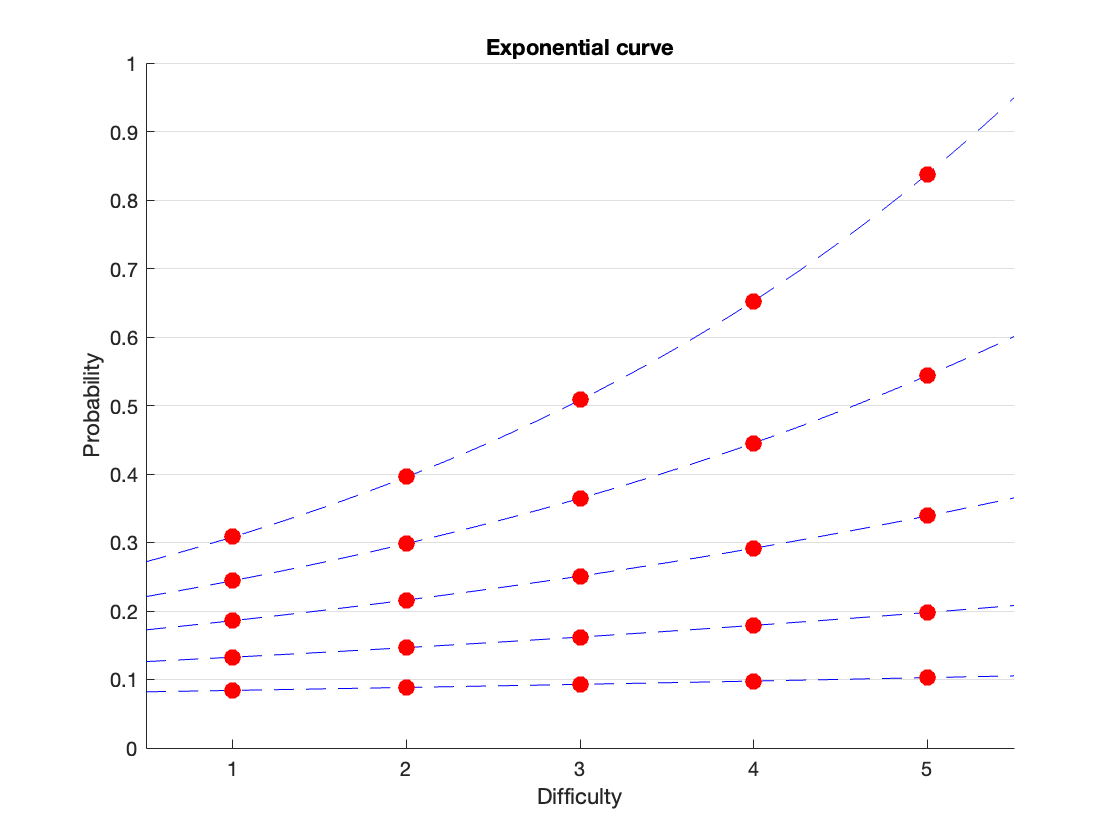
\includegraphics[width=\linewidth]{exp.png}
        \caption{Five possible learning curves following the exponential equation $\vartheta(d) = ae^{b(d-1)}$.}
        \label{exp1}
    \end{subfigure}\hspace{0.05\linewidth}
    \begin{subfigure}[b]{0.4\linewidth}
        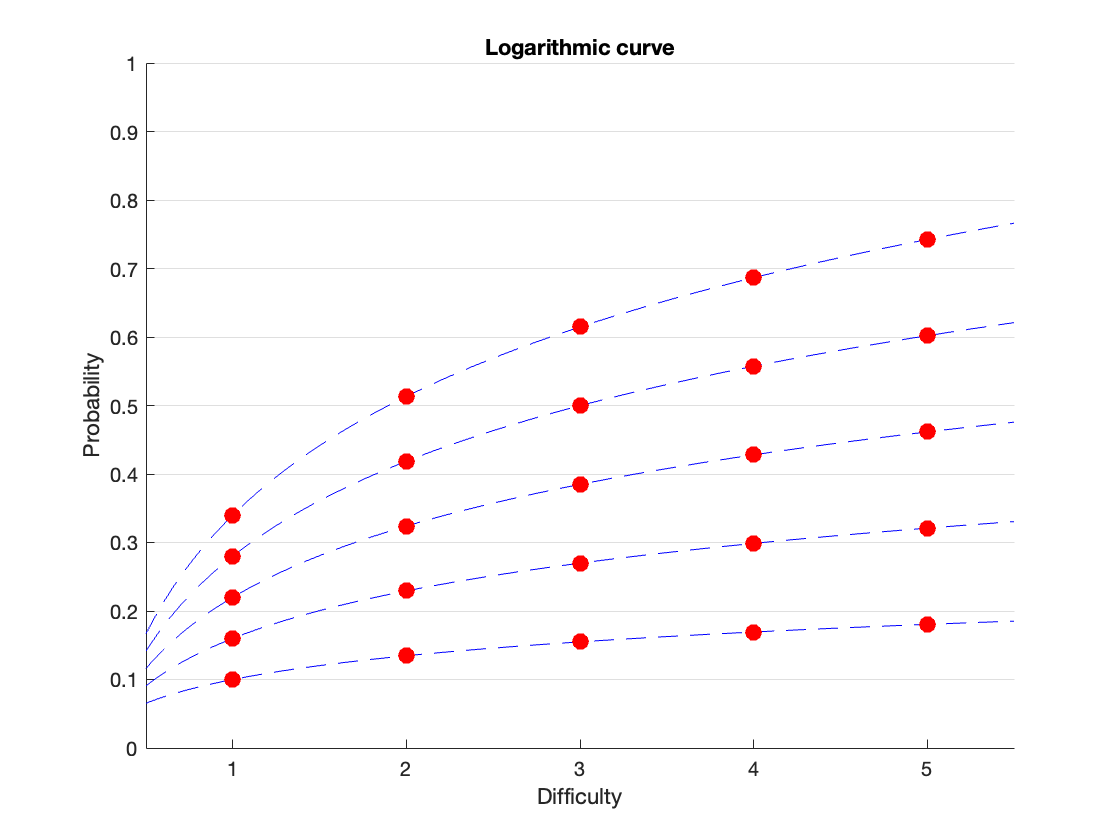
\includegraphics[width=\linewidth]{log.png}
        \caption{Five possible learning curves following the logarithmic equation $\vartheta(d) = a + b\ln d$.}
        \label{log1}
    \end{subfigure}
    \caption{Predictions of the \textsl{exponential} \eqref{exp1} and the \textsl{logarithmic} \eqref{log1} curves.}
    \label{fig1}
\end{figure}

After computing all the learning curves, it is possible to make exponential and logarithmic regressions on those curves, to find the parameters $a$ and $b$.
Then, the residuals are calculated and the regression with smaller residuals gets assigned to the learning curve.
Finally, to get two variables within the same range of values, $\openinter{0}{1}$, we retrieve the value $a$ and the value $b'=-\frac{4b}{\ln a}$, for \eqref{eqexp}, or $b'=\frac{b\ln 5}{1-a}$, for \eqref{eqlog}.

\section{Tendency distribution}
Imagine you want to model a tendency, consisting on one specific task $t$ at a time. Moreover, the probability of not succeeding on that task, $s$, called \textsl{slip}, influences whether or not $t$ is completed everytime.
That said, the probability of succeeding on one task is $p(x) = (1-s)^{x}s^{1-x}$, with $x \in \{0,1\}$. If we regard each task as an independent variate, with fixed probability, then $p({\bf v}) = \prod_{i=1}^{n}(1-s)^{v_i}s^{1-v_i}$, with ${\bf v} = \{0,1\}^n$.
However, since we want to model tendencies, each task will have a different impact on the overall probability, proportional to their frequency of successes. This way, instead of multiplying all probabilities individually, we sum them with predetermined weights, and normalize so all possible outcomes sum up to 1.
So the formula is of the form
\begin{equation}
    p({\bf v}) = \frac{\sum_{i=1}^{n}\gamma_i(1-s)^{v_i}s^{1-v_i}}{C(n)\cdot\sum_{i=1}^{n}\gamma_i},\label{eqtendency1}
\end{equation}
with $C(n)\colon \mathbb{N} \longrightarrow \mathbb{R}$, $\forall i,j ~ \gamma_i\gamma_j \ge 0$ and ${\boldsymbol \gamma} \ne \0_n$. Also, we force $\forall i,j ~ \gamma_i\gamma_j \ge 0$ to guarantee that $p({\bf v})$ only returns values between $0$ and $1$.
\begin{theorem} \label{sumtheo}
    Regarding the equation \eqref{eqtendency1}, exists $C(n)\colon \mathbb{N} \longrightarrow \mathbb{R}$ such that,
    \begin{equation*}
        {\boldsymbol \gamma} \ne \0_n \Rightarrow \sum_{{\bf v} \in \{0,1\}^n}p({\bf v}) = 1.
    \end{equation*}
\end{theorem}
\begin{proof}
    First we need to convert the equation \eqref{eqtendency1} into its matrix form.
    \begin{alignat}{2}
        {\bf v}_i \in \{0,1\} \mkern5mu&&\Rightarrow\mkern5mu (1-s)^{v_i}s^{1-v_i} &= v_i(1-s) + s(1-v_i) \notag \\
        \LRA && \sum_{i=1}^{n}\gamma_i(1-s)^{v_i}s^{1-v_i} &= \begin{bmatrix}
            v_1(1-2s) + s & v_2(1-2s) + s & \dots & v_n(1-2s) + s
        \end{bmatrix} \begin{bmatrix}
            \gamma_1 \\ \gamma_2 \\ \vdots \\ \gamma_n
        \end{bmatrix} \notag \\
        &&&= \left((1-2s)\cdot {\bf v}\T + s\cdot\1_n\T\right)\cdot {\boldsymbol \gamma}. \label{step1}
    \end{alignat}
    \begin{equation}
        C(n)\cdot\sum_{i=1}^{n}\gamma_i = C(n) \cdot \1_n\T \cdot {\boldsymbol \gamma}. \label{step2}
    \end{equation}
    Combining \eqref{step1} and \eqref{step2},
    \begin{equation}
        p({\bf v}) = \frac{\left((1-2s)\cdot {\bf v}\T + s\cdot\1_n\T\right)\cdot {\boldsymbol \gamma}}{C(n) \cdot \1_n\T \cdot {\boldsymbol \gamma}}.
    \end{equation}
    To prove the theorem, we have to sum all values of $p({\bf v})$, where ${\bf v} \in \{0,1\}^n$, and find for what values of $C(n)$ the statement $\sum_{{\bf v} \in \{0,1\}^n} p({\bf v}) = 1$. For that, lets consider the matrix $\V_n$ where every row is an unique vector ${\bf v}_i \in \{0,1\}^n$, that is, $\V_n \in \left\{0,1\right\}^{2^n \times n}$ such as
    $$ \V_n = \begin{bmatrix}
        {\bf v}_1 & {\bf v}_2 & \dots & {\bf v}_{2^n}
    \end{bmatrix}\T.  $$
    With ${\boldsymbol \gamma} \ne \0_n$,
    \begin{align*}
        \sum_{{\bf v} \in \{0,1\}^n} p({\bf v}) &= \frac{\sum_{{\bf v} \in \{0,1\}^n}\left((1-2s)\cdot {\bf v}\T + s\cdot\1_n\T\right)\cdot {\boldsymbol \gamma}}{C(n) \cdot \1_n\T \cdot {\boldsymbol \gamma}} \\
        &= \frac{\left((1-2s)\cdot\1\T_{\left\lvert \{0,1\}^n \right\rvert} \cdot \V_n + s\left\lvert \{0,1\}^n \right\rvert\cdot \1_n\T \right)\cdot {\boldsymbol \gamma}}{C(n) \cdot \1_n\T \cdot {\boldsymbol \gamma}} \\
        &= \frac{\left(2^{n-1}(1-2s)\cdot\1_n\T + 2^ns\cdot\1_n\T\right)\cdot {\boldsymbol \gamma}}{C(n) \cdot \1_n\T \cdot {\boldsymbol \gamma}} \\
        &= \frac{2^{n-1}\cdot\1_n\T\cdot{\boldsymbol \gamma}}{C(n) \cdot \1_n\T \cdot {\boldsymbol \gamma}} \\
        &= \frac{2^{n-1}}{C(n)}.
    \end{align*}
    If we set $C(n) = 2^{n-1}$, then $\sum_{{\bf v} \in \{0,1\}^n} p({\bf v}) = 1$ holds for any $\gamma_i \in \mathbb{R}^+_0$ such that ${\boldsymbol \gamma} \ne \0_n$.
\end{proof}
Based on the above theorem, let's start defining our tendency distribution. Let $V \sim \Tend{s}{\boldsymbol \gamma}$ be a vector-valued random variate, that follows a tendency distribution, where $s$ represents the \textsl{slip}, $n$ is the number of trials and ${\boldsymbol \gamma}$ is the weights vector, such that $\forall i,j ~ \gamma_i\gamma_j \ge 0$ and ${\boldsymbol \gamma} \ne \0_n$.
We can start by defining the probability density function (PDF): 
\begin{align}
    \begin{split}
        f\colon \left\{0,1\right\}^n &\longrightarrow \left[0,1\right] \\
        {\bf v} &\longmapsto \frac{\left(\left(1-2s\right) \cdot {\bf v}\T + s\cdot\1_n\T\right) \cdot {\boldsymbol \gamma}}{2^{n-1}\cdot \1_n\T \cdot {\boldsymbol \gamma}}.
    \end{split} \label{pdf}
\end{align}
\begin{theorem} \label{expvartheo1}
    Regarding the PDF \eqref{pdf}, and the random variate $V \sim \textup{Tend}(s, {\boldsymbol \gamma})$, the expected value and scalar variance are:
    \begin{align}
        \textup{E}[V] &= \frac{1}{2}\left(\frac{1-2s}{\1_n\T\cdot {\boldsymbol \gamma}}\cdot {\boldsymbol \gamma} + \1_n\right), \label{expected} \\
        \textup{Var}[V] &= \frac{1}{2}\left(\1_n - \frac{1-2s}{\1_n\T\cdot {\boldsymbol \gamma}}\cdot {\boldsymbol \gamma}\right)\T \cdot \textup{E}[V]. \label{variance}
    \end{align}
\end{theorem}
\begin{proof}
    To prove the expected value, we just need to use algebra to achieve the answer. 
    \begin{align*}
        \text{E}[V] &= \sum_{{\bf v} \in \left\{0,1\right\}^n} f({\bf v})\cdot {\bf v} \\
        &= \V_n\T \cdot {\bf f}(\V_n),
    \end{align*}
    where ${\bf f}$ is the matrix representation of the PDF $f$, for all possible values of ${\bf v} \in \left\{0,1\right\}^n$. Since $\V_n$ is constructed such as all possible values ${\bf v}$ are distributed on the rows, we just need to change ${\bf v}\T$ to $\V_n$ and $\1_n\T$ to $\1_{2^n\times n}$ in $f$. This way,
    \begin{equation*}
        {\bf f}(\V_n) = \frac{\left(\left(1-2s\right) \cdot \V_n + s\cdot\1_{2^n\times n}\right)\cdot {\boldsymbol \gamma} }{2^{n-1}\cdot \1_n\T \cdot {\boldsymbol \gamma}}.
    \end{equation*}
    Using this result,
    \begin{align*}
        \text{E}[V] &= \V_n\T \cdot {\bf f}(\V_n) \\
        &= \frac{\V_n\T \cdot \left(\left(1-2s\right) \cdot \V_n + s\cdot\1_{2^n\times n}\right)\cdot {\boldsymbol \gamma} }{2^{n-1}\cdot \1_n\T \cdot {\boldsymbol \gamma}} \\
        &= \frac{\left(\left(1-2s\right) \cdot \V_n\T \cdot  \V_n + s\cdot\V_n\T \cdot \1_{2^n\times n}\right)\cdot {\boldsymbol \gamma} }{2^{n-1}\cdot \1_n\T \cdot {\boldsymbol \gamma}}.
    \end{align*}
    By the properties of the matrix $\V_n$, we can calculate $\V_n\T\cdot\V_n = 2^{n-2}\left(I_n + \1_{n\times n}\right) $, where $I_n = \diag{\1_n}$ is the identity matrix of size $n$, and $\V_n\T\cdot\1_{2^n\times n} = 2^{n-1}\cdot\1_{n\times n} = 2\left(2^{n-2}\cdot\1_{n\times n}\right) $. So,
    \begin{align*}
        \text{E}[V] &= \frac{\left(2^{n-2}(1-2s)I_n + (1-2s)\left(2^{n-2}\cdot\1_{n\times n}\right) + 2s\left(2^{n-2}\cdot\1_{n\times n}\right) \right)\cdot {\boldsymbol \gamma} }{2^{n-1}\cdot \1_n\T \cdot {\boldsymbol \gamma}} \\
        &= \frac{\left((1-2s)I_n + \1_{n\times n}\right) \cdot {\boldsymbol \gamma}}{2\cdot \1_n\T \cdot {\boldsymbol \gamma}} \\
        &= \frac{1}{2}\left(\frac{1-2s}{\1_n\T \cdot {\boldsymbol \gamma}}\cdot {\boldsymbol \gamma} + \frac{\1_n\cdot\1_n\T\cdot {\boldsymbol \gamma}}{\1_n\T\cdot {\boldsymbol \gamma}}\right)  \\
        &= \frac{1}{2}\left(\frac{1-2s}{\1_n\T\cdot {\boldsymbol \gamma}}\cdot {\boldsymbol \gamma} + \1_n\right),
    \end{align*}
    proving \eqref{expected}. For the variance, we define ${\boldsymbol \mu} = \text{E}[V]$ and the definition for vector-valued random variates $\text{Var}[V] = \text{E}\left[\left(V-{\boldsymbol \mu}\right)\T\left(V-{\boldsymbol \mu}\right)\right]$ to find the result.
    \begin{align*}
        \text{Var}[V] &= \text{E}\left[\left(V-{\boldsymbol \mu}\right)\T\left(V-{\boldsymbol \mu}\right)\right] \\
        &= \sum_{{\bf v} \in \left\{0,1\right\}^n} f({\bf v}) \cdot \left({\bf v}-{\boldsymbol \mu}\right)\T\left({\bf v}-{\boldsymbol \mu}\right) \\
        &= \sum_{{\bf v} \in \left\{0,1\right\}^n} f({\bf v}) R({\bf v}) \\
        &= \Diag{{\bf R}(\V_n)}\T \cdot {\bf f}(\V_n),
    \end{align*}
    where $ R({\bf v}) = \left({\bf v}-{\boldsymbol \mu}\right)\T\left({\bf v}-{\boldsymbol \mu}\right) $, $\Diag{M} = (M \circ I_n)\cdot\1_n$ is a linear function that returns the diagonal of a matrix as a column vector, and ${\bf R}$ is the matrix representation of the function $R$ for all possible values of ${\bf v} \in \left\{0,1\right\}^n$.
    We now have to find $\Diag{{\bf R}(\V_n)}$. Similarly to ${\bf f}$, if $R$ uses the unique vector as a column, in the matrix representation we replace it with $\V_n\T$. To respect the matrix dimensions, we need to extend the vector ${\boldsymbol \mu}$ to the matrix ${\boldsymbol \mu}\cdot\1_{2^n}\T$. This way,
    \begin{equation*}
        {\bf R}(\V_n) = \left(\V_n\T - {\boldsymbol \mu}\cdot\1_{2^n}\T\right)\T\left(\V_n\T - {\boldsymbol \mu}\cdot\1_{2^n}\T\right).
    \end{equation*}
    Due to the distributive property of matrices and the linearity of the Diag function,
    \begin{align*}
        \Diag{{\bf R}(\V_n)} &= \Diag{\V_n\cdot\1_n\T - \left(\V_n\cdot{\boldsymbol \mu}\cdot\1_{2^n}\T\right)\T - \V_n\cdot{\boldsymbol \mu}\cdot\1_{2^n}\T + {\boldsymbol \mu}^2\cdot\1_{2^n \times 2^n}}. \\
        \Diag{\V_n\cdot\1_n\T} &= \V_n\cdot\1_n, \\
        \Diag{\left(\V_n\cdot{\boldsymbol \mu}\cdot\1_{2^n}\T\right)\T } &= \Diag{\V_n\cdot{\boldsymbol \mu}\cdot\1_{2^n}\T}, \\
        \Diag{\V_n\cdot{\boldsymbol \mu}\cdot\1_{2^n}\T} &= \V_n\cdot{\boldsymbol \mu}, \\
        \Diag{\1_{2^n \times 2^n}} &= \1_{2^n},
    \end{align*}
    where ${\boldsymbol \mu}^2 = {\boldsymbol \mu}\T\cdot {\boldsymbol \mu} = \left\lVert {\boldsymbol \mu}\right\rVert^2$, which means,
    \begin{align}
        \Diag{{\bf R}(\V_n)} &= \V_n\cdot\1_n - 2\cdot\V_n\cdot{\boldsymbol \mu} + {\boldsymbol \mu}^2\cdot\1_{2^n} \\
        &= \V_n\cdot\left(\1_n - 2\cdot{\boldsymbol \mu}\right) + {\boldsymbol \mu}^2\cdot\1_{2^n}.
    \end{align}
    Before finishing the proof, we present some auxiliary results, important to some steps of the calculations.
    \begin{align*}
        \left(\1_n - 2\cdot{\boldsymbol \mu}\right) &= -\frac{1-2s}{\1_n\T\cdot{\boldsymbol \gamma}}\cdot{\boldsymbol \gamma}, \\
        {\boldsymbol \mu}^2 &= \frac{1}{4}\left(\frac{1-2s}{\1_n\T\cdot {\boldsymbol \gamma}}\cdot {\boldsymbol \gamma} + \1_n\right)^2 = \frac{1}{4}\left(\frac{1-2s}{\1_n\T\cdot {\boldsymbol \gamma}}\cdot {\boldsymbol \gamma}\right)^2 + \frac{1-2s}{2} + \frac{1}{4}\left(\1_n\right)^2, \\
        \1_{2^n}\T\cdot\1_{2^n\times n} &= 2^n \cdot \1_n\T = 2\left(2^{n-1} \cdot \1_n\T \right), \\
        \1_{2^n}\T\cdot\V_n &= 2^{n-1} \cdot \1_n\T.
    \end{align*}
    We can now find the value for the variance.
    \begin{align*}
        \text{Var}[V] &= \Diag{{\bf R}(\V_n)}\T \cdot {\bf f}(\V_n) \\
        &= \frac{\left(\V_n\cdot\left(\1_n - 2\cdot{\boldsymbol \mu}\right) + {\boldsymbol \mu}^2\cdot\1_{2^n}\right)\T \cdot \left(\left(1-2s\right) \cdot \V_n + s\cdot\1_{2^n\times n}\right)\cdot {\boldsymbol \gamma}}{2^{n-1}\cdot \1_n\T \cdot {\boldsymbol \gamma}} \\
        &= \frac{\left[
            (1-2s)\left(\1_n - 2{\boldsymbol \mu}\right)\T\V_n\T\V_n
            + s\left(\1_n - 2{\boldsymbol \mu}\right)\T\V_n\T\1_{2^n\times n}
            + (1-2s){\boldsymbol \mu}^2\1_{2^n}\T\V_n
            + s{\boldsymbol \mu}^2\1_{2^n}\T\1_{2^n\times n}
        \right] \cdot {\boldsymbol \gamma} }{2^{n-1}\cdot \1_n\T \cdot {\boldsymbol \gamma}} \\
        &= \frac{\left[
            2^{n-2}(1-2s)\left(\1_n - 2{\boldsymbol \mu}\right)\T\cdot I_n
            + \left(\1_n - 2{\boldsymbol \mu}\right)\T\left(2^{n-2}\cdot\1_{n\times n}\right)
            + 2^{n-1}{\boldsymbol \mu}^2\1_n\T
        \right] \cdot {\boldsymbol \gamma} }{2^{n-1}\cdot \1_n\T \cdot {\boldsymbol \gamma}} \\
        &= \frac{\left[
            (1-2s)\left(\1_n - 2{\boldsymbol \mu}\right)\T\cdot I_n
            + \left(\1_n - 2{\boldsymbol \mu}\right)\T\cdot\1_{n\times n}
            + 2{\boldsymbol \mu}^2\1_n\T
        \right] \cdot {\boldsymbol \gamma} }{2\cdot \1_n\T \cdot {\boldsymbol \gamma}} \\
        &= \frac{-\frac{(1-2s)^2}{\1_n\T\cdot{\boldsymbol \gamma}}\cdot {\boldsymbol \gamma}\T{\boldsymbol \gamma} - (1-2s)\cdot\1_n\T\cdot{\boldsymbol \gamma} + 2{\boldsymbol \mu}^2\cdot\1_n\T\cdot{\boldsymbol \gamma}}{2\cdot \1_n\T \cdot {\boldsymbol \gamma}} \\
        &= -\frac{1}{2}\left(\frac{1-2s}{\1_n\T\cdot {\boldsymbol \gamma}}\cdot {\boldsymbol \gamma}\right)^2 + \frac{\left(-(1-2s) + 2{\boldsymbol \mu}^2\right) \cdot \1_n\T\cdot {\boldsymbol \gamma} }{2\cdot \1_n\T \cdot {\boldsymbol \gamma}} \\
        &= -\frac{1}{2}\left(\frac{1-2s}{\1_n\T\cdot {\boldsymbol \gamma}}\cdot {\boldsymbol \gamma}\right)^2 + \frac{-(1-2s) + \frac{1}{2}\left(\frac{1-2s}{\1_n\T\cdot {\boldsymbol \gamma}}\cdot {\boldsymbol \gamma}\right)^2 + (1-2s) + \frac{1}{2}\cdot\left(\1_n\right)^2}{2} \\
        &= \frac{1}{4}\left(\left(\1_n\right)^2 - \left(\frac{1-2s}{\1_n\T\cdot {\boldsymbol \gamma}}\cdot {\boldsymbol \gamma}\right)^2 \right) \\
        &= \frac{1}{2}\left(\1_n - \frac{1-2s}{\1_n\T\cdot {\boldsymbol \gamma}}\cdot {\boldsymbol \gamma}\right)\T \cdot \text{E}[V],
    \end{align*}
    proving \eqref{variance}.
\end{proof}
It's easy to notice that both $\text{E}[V]$ and $\text{Var}[V]$ have a common expression, that we'll call ${\boldsymbol \rho}$, and
\begin{align*}
    {\boldsymbol \rho} &= \frac{1-2s}{\1_n\T\cdot {\boldsymbol \gamma}}\cdot {\boldsymbol \gamma}, \\
    \textup{E}[V] &= \frac{1}{2}\left(\1_n + {\boldsymbol \rho}\right) , \\
    \textup{Var}[V] &= \frac{1}{4}\left(\1_n - {\boldsymbol \rho}\right)\T\left(\1_n + {\boldsymbol \rho}\right) = \frac{1}{4}\left(n - {\boldsymbol \rho}^2\right)  ,
\end{align*}
and $s \lesseqqgtr \frac{1}{2} \Rightarrow {\boldsymbol \rho} \gtreqqless \0_n$. 
Before looking into the statistical inference of this model, we need to state the following lemma and theorem.
\begin{lemma} \label{lemma1}
    Let $T({\boldsymbol \gamma}) = \frac{1-2s}{\1_n\T\cdot {\boldsymbol \gamma}}$. So ${\boldsymbol \rho} = T({\boldsymbol \gamma})\cdot {\boldsymbol \gamma}$, and
    \begin{equation*}
        s \ne \frac{1}{2} \Rightarrow {\boldsymbol \rho} = T({\boldsymbol \rho}) \cdot {\boldsymbol \rho}.
    \end{equation*}
\end{lemma}
\begin{proof}
    \begin{alignat*}{2}
        && {\boldsymbol \rho} &= T({\boldsymbol \rho}) \cdot {\boldsymbol \rho} \\
        \LRA && 1 &= T({\boldsymbol \rho}) \\
        \LRA && 1 &= \frac{1-2s}{\1_n\T\cdot {\boldsymbol \rho}} \\
        \LRA && 1 &= \frac{1-2s}{\1_n\T\cdot \left(T({\boldsymbol \gamma})\cdot {\boldsymbol \gamma}\right) } \\
        \LRA && 1 &= \frac{1-2s}{\1_n\T\cdot \left(\frac{1-2s}{\1_n\T\cdot {\boldsymbol \gamma}}\cdot {\boldsymbol \gamma}\right) } \\
        \LRA && 1 &= \frac{1-2s}{1-2s} \\
        \LRA && 1 &= 1,
    \end{alignat*}
    that holds if $1-2s \ne 0 \Leftrightarrow s \ne \frac{1}{2}$.
\end{proof}
The proof of this lemma shows that ${\boldsymbol \rho}$ is a fixed-point just after one iteration, using ${\boldsymbol \gamma}$ as starting weights vector.
\begin{theorem}
    Let ${\boldsymbol \rho} = T({\boldsymbol \gamma})\cdot {\boldsymbol \gamma}$ and $V \sim \textup{Tend}(s, {\boldsymbol \gamma})$ a random variate. So
    \begin{equation*}
        \hat{f}({\bf v}) = \frac{\left(\left(1-2s\right) \cdot {\bf v}\T + s\cdot\1_n\T\right) \cdot {\boldsymbol \rho}}{2^{n-1}\cdot \1_n\T \cdot {\boldsymbol \rho}}
    \end{equation*}
    is also a PDF for $V$ and $\hat{f} \cong f$.
\end{theorem}
\begin{proof}
    By the same proof of the theorem \ref{sumtheo}, we can conclude that $\sum_{{\bf v} \in \left\{0,1\right\}^n} \hat{f}({\bf v}) = 1$.
    Now let's divide the proof in two cases. First, if $s = \frac{1}{2}$, then
    $$ \hat{f}({\bf v}) = \frac{1}{2^n}, $$
    which means the PDF is independent of both the vectors ${\bf v}$ and ${\boldsymbol \rho}$, and holds the characteristics of the PDF.

    If $s \ne \frac{1}{2}$, by the proof ot the theorem \ref{expvartheo1}, we achieve
    \begin{align*}
        \hat{\boldsymbol \rho} &= \frac{1-2s}{\1_n\T\cdot {\boldsymbol \rho}}\cdot {\boldsymbol \rho} = T({\boldsymbol \rho}) \cdot {\boldsymbol \rho}, \\
        \widehat{\text{E}}[V] &= \frac{1}{2}\left(\1_n + \hat{\boldsymbol \rho}\right) , \\
        \widehat{\text{Var}}[V] &= \frac{1}{4}\left(\1_n - \hat{\boldsymbol \rho}'\right)\T\left(\1_n + \hat{\boldsymbol \rho}'\right).
    \end{align*}
    However, by the lemma \ref{lemma1}, ${\boldsymbol \rho} = T({\boldsymbol \rho}) \cdot {\boldsymbol \rho} = \hat{\boldsymbol \rho}$, which means $\widehat{\text{E}}[V] = \text{E}[V]$ and $\widehat{\text{Var}}[V] = \text{Var}[V]$, thus proving that $\hat{f}$ is also a PDF for $V$, that retains the same expected value and scalar variance.

    Furthermore, $\hat{f} \cong f$ because
    \begin{align*}
        \hat{f}({\bf v}) &= \frac{\left(\left(1-2s\right) \cdot {\bf v}\T + s\cdot\1_n\T\right) \cdot {\boldsymbol \rho}}{2^{n-1}\cdot \1_n\T \cdot {\boldsymbol \rho}} \\
        &= \frac{\left(\left(1-2s\right) \cdot {\bf v}\T + s\cdot\1_n\T\right) \cdot \left(T({\boldsymbol \gamma})\cdot {\boldsymbol \gamma}\right) }{2^{n-1}\cdot \1_n\T \cdot \left(T({\boldsymbol \gamma})\cdot {\boldsymbol \gamma}\right)} \\
        &= \frac{\left(\left(1-2s\right) \cdot {\bf v}\T + s\cdot\1_n\T\right) \cdot {\boldsymbol \gamma}}{2^{n-1}\cdot \1_n\T \cdot {\boldsymbol \gamma}} \\
        &= f({\bf v}),
    \end{align*}
    when $s \ne \frac{1}{2}$ and,
    $$ \hat{f}({\bf v}) = \frac{1}{2^n} = f({\bf v}), $$
    when $s = \frac{1}{2}$.
\end{proof}

\subsection{Statistical Model and Inference}
By the properties of the tendency distribution's PDF, the vector ${\bf v} = \1_n$ corresponds to either the greastest probability or the lowest, if $s < \frac{1}{2}$ or $s > \frac{1}{2}$, respectively.
But how is it possible that the vector where every outcome is successful is either the most or the least probable? It makes sense in the same way a chain of Bernoulli events also give the greatest or lowest probability when all tasks are successful, based on the value of its parameter.
Moreover, in a tendency distribution, the goal is to get the most successes possible, and the weights only state the importance of a specific task to the overall probability; a task that is usually failed will have a lower weight and thus succeeding or failing doesn't affect much the probability of that vector amongst the data.

To look into the statistical model, we first introduce the function $\varGamma({\boldsymbol \gamma}) = T({\boldsymbol \gamma})\cdot {\boldsymbol \gamma}$, noting that ${\boldsymbol \rho} = \varGamma({\boldsymbol \rho})$. This function has degree 0 of homogeneity, because $\varGamma( t \cdot{\boldsymbol \gamma}) = \varGamma({\boldsymbol \gamma}) = {\boldsymbol \rho}$.

Suppose $V = \left(V_1, V_2, \dots, V_k\right)$ are independent and identically distributed (i.i.d.) random variates, such that $V_i \sim \Tend{s}{\boldsymbol \gamma}$, with known \textsl{slip} and unknown weights. How can one estimate the value of the weights parameter?
Following the empirical frequency of successes of each task on all samples, we can set the estimator
\begin{equation}
    \widehat{\boldsymbol \rho}(V) = \varGamma(V\cdot\1_k). \label{esti}
\end{equation}
Now we calculate how biased is this estimator, and the mean difference between the coordinates of the estimator and the true weights. Note that, for approximation purposes, the denominator $\1_n\T \cdot V \cdot \1_k$ loses sense on the calculations, so we replace it for the constant $\alpha$, that accounts for the total number of successful tasks in all observations of $V$.
\begin{align*}
    \text{E}\left[\widehat{\boldsymbol \rho}(V)\right] &= \text{E}\left[\varGamma(V\cdot\1_k)\right] \\
    &= \text{E}\left[\frac{1-2s}{\alpha}\sum_{i=1}^{k}V_i\right] \\
    &= \frac{k(1-2s)}{\alpha}\text{E}\left[V\right] \\
    &= \frac{k(1-2s)}{2\alpha}(\1_n + {\boldsymbol \rho}),
\end{align*}
making the $\text{Bias}(\widehat{\boldsymbol \rho}) = \frac{k(1-2s)}{2\alpha}(\1_n + {\boldsymbol \rho}) - {\boldsymbol \rho}$. Now we calculate the mean of each weight of the bias.
\begin{align*}
    \text{MSD}\left(\widehat{\boldsymbol \rho}(V)\right) &= \frac{1}{n}\1_n\T\cdot\left(\frac{k(1-2s)}{2\alpha}(\1_n + {\boldsymbol \rho}) - {\boldsymbol \rho}\right) \\
    &= \frac{1}{n}\left[\frac{k(1-2s)}{2\alpha}\left(\1_n\T\cdot\1_n + \1_n\T\cdot{\boldsymbol \rho}\right) - \1_n\T\cdot{\boldsymbol \rho}\right]  \\
    &= \frac{1}{n}\left[\frac{k(1-2s)}{2\alpha}\left(n + (1-2s)\right) - (1-2s)\right] \\
    &= \frac{1-2s}{n}\left[\frac{k}{2\alpha}\left(n + (1-2s)\right) - 1\right].
\end{align*}
This result shows that with greater values of $n$, the closer to $0$ is $\text{MSD}\left(\widehat{\boldsymbol \rho}(V)\right)$, because (and supposing the observations of $V$ have little to none $\0_n$ vectors) $\alpha$ is almost everytime greater than $k$, and $\alpha \le nk$.
Similarly, as $\alpha \to nk$, $\text{MSD}\left(\widehat{\boldsymbol \rho}(V)\right) \to \frac{(1-2s)(1-2s-n)}{2n^2}$, that approaches $0$ when $n \to +\infty$.
So this makes our estimator \eqref{esti} a good enought approximation of the ideal weigths vector for the tendency distributions.

Knowing now the weigths vector, there is a simple way to apply inference to the parameter.
Let $V^1 = \left(V_1, \dots, V_i\right)$, $V^2 = \left(V_{i+1}, \dots, V_k\right)$ and $V = \left(V^1, V^2\right)$ be i.d.d. random variates, where $V^1_j \sim \Tend{s}{\boldsymbol \rho}$, with known \textsl{slip} and weights, $V^2_j \sim \Tend{s}{\widetilde{\boldsymbol \rho}}$, with known \textsl{slip} and unknown weights, and $V_j \sim \Tend{s}{\widehat{\boldsymbol \rho}}$, with known \textsl{slip} and unknown weights.
Regarding the previous estimator,
\begin{align*}
    \widehat{\boldsymbol \rho}(V) &= \varGamma(V\cdot\1_k) \\
    &= \varGamma((V^1 + V^2)\cdot\1_k) \\
    &= \frac{(1-2s)\cdot (V^1 + V^2)\cdot\1_k}{\1_n\T\cdot(V^1 + V^2)\cdot\1_k} \\
    &= (1-2s)\frac{V^1\cdot\1_k + V^2\cdot\1_k}{\1_n\T\cdot V^1\cdot\1_k + \1_n\T\cdot V^2\cdot\1_k} \\
    &= (1-2s)\left(\frac{V^1\cdot\1_k}{\1_n\T\cdot V^1\cdot\1_k} \oplus \frac{V^2\cdot\1_k}{\1_n\T\cdot V^2\cdot\1_k}\right) \\
    &= \varGamma(V^1\cdot\1_k) \oplus \varGamma(V^2\cdot\1_k) \\
    &= {\boldsymbol \rho}(V^1) \oplus \widetilde{\boldsymbol \rho}(V^2),
\end{align*}
where the operation $\oplus$ is the Farey sum, and $s \in [0,1] \cap \mathbb{Q} \setminus \left\{\frac{1}{2}\right\}$. This means that, having the weights vector for $V^1$ and estimating the weights vector for $V^2$, we can apply inference to update the weights for $V$.

\subsection{Model Predictions}
The fact that a tendency distribution has a fixed size $n$ for each sample can be used as an advantage to model structures of fixed size.
For this web application, the structure consists of the questions of a given topic, and each sample saves the first attempt of a student on all the questions, where $1$ is a wrong answer and $0$ otherwise.



\section{Routine Distribution}
Another way of modelling tendencies is with the creation of routines with greater periods, where the vector ${\bf v}$ that best fits that routine will have a greater probability. Following a similar weights approach, instead of multiplying the weights to each probability, the weight determines the probability and they are all multiplied together.
So the formula is of the form
\begin{equation}
    p({\bf v}) = \frac{\prod_{i=1}^{n}\gamma_i^{v_i}}{C(\gamma)}, \label{eqtendency2}
\end{equation}
with $C\colon \left(\mathbb{R}^+\right)^n \longrightarrow \mathbb{R}^+$ and $\gamma_i \in \mathbb{R}^+$. We also force $p\colon \left\{0,1\right\}^n \longrightarrow \left[0,1\right]$.

\begin{theorem}
    Regarding the equation \eqref{eqtendency2}, exists $C\colon \left(\mathbb{R}^+\right)^n \longrightarrow \mathbb{R}^+$ such that, for all $\gamma_i \in \mathbb{R}^+$, $$\sum_{{\bf v} \in \{0,1\}^n}p({\bf v}) = 1.$$
\end{theorem}
\begin{proof}
    Since $C(\gamma)$ does not depend on ${\bf v}$,
    \begin{align*}
        \sum_{{\bf v} \in \{0,1\}^n}p({\bf v}) &= \sum_{{\bf v} \in \{0,1\}^n}\frac{\prod_{i=1}^{n}\gamma_i^{v_i}}{C(\gamma)} \\
        &= \frac{\sum_{{\bf v} \in \{0,1\}^n}\prod_{i=1}^{n}\gamma_i^{{\bf v}_i}}{C(\gamma)}.
    \end{align*}
    Due to the binary properties of the vector ${\bf v}$, and since we iterate over all possible values of ${\bf v} \in \{0,1\}^n$, we can rewrite
    \begin{equation*}
        \sum_{{\bf v} \in \{0,1\}^n}\prod_{i=1}^{n}\gamma_i^{v_i} = \prod_{i=1}^{n}(1+\gamma_i).
    \end{equation*}
    Replacing this result,
    \begin{equation*}
        \sum_{{\bf v} \in \{0,1\}^n}p({\bf v}) = \frac{\prod_{i=1}^{n}(1+\gamma_i)}{C(\gamma)}.
    \end{equation*}
    If we set $C(\gamma) = \prod_{i=1}^{n}(1+\gamma_i)$, then $\sum_{{\bf v} \in \{0,1\}^n}p({\bf v}) = 1$, for all $\gamma_i \in \mathbb{R}^+$.
\end{proof}
So let's define our routine distribution. Let $V \sim \Rout{\boldsymbol \gamma}$ be a vector-valued random variate, that follows a routine distribution, where $n$ is the number of trials and ${\boldsymbol \gamma} \in \left(\mathbb{R}^+\right)^n$ is the weights vector.
We can start by defining the probability density function (PDF):
\begin{align}
    \begin{split}
        f\colon \left\{0,1\right\}^n &\longrightarrow \left[0,1\right] \\
        {\bf v} &\longmapsto \prod_{i=1}^{n}\frac{\gamma_i^{v_i}}{1+\gamma_i}.
    \end{split} \label{pdf2}
\end{align}
Before converting the PDF to its matrix form, we need to revisit the definition of the function $\varpi$. Above, we have described $\varpi_r(b) = \det\!\left(\diag{b}\right)$, but we need to extend this function to accept also matrices. So we will call this method the hadamard matrix compression (by rows or columns), where given the matrices $M$ and $N$ and such that,
\begin{align*}
    M &= \begin{bmatrix}
        {\bf v}_1 & {\bf v}_2 & \dots & {\bf v}_n
    \end{bmatrix}, \\
    N &= \begin{bmatrix}
        {\bf w}_1 & {\bf w}_2 & \dots & {\bf w}_n
    \end{bmatrix}\T,
\end{align*}
the functions $\varpi_c$ and $\varpi_r$ are defined as
\begin{align*}
    \varpi_c(M) &= {\bf v}_1 \circ {\bf v}_2 \circ \dots \circ {\bf v}_n, \\
    \varpi_r(N) &= {\bf w}_1\T \circ {\bf w}_2\T \circ \dots \circ {\bf w}_n\T, \\
    \varpi_c(M) &= \varpi_r(M\T)\T.
\end{align*}
Now, after some simple calculations, it is possible to define the PDF in its matrix form:
\begin{equation}
    f({\bf v}) = \varpi_r\left(\left({\bf v}\circ\left({\boldsymbol \gamma} - \1_n\right) + \1_n\right)\circ \left(\1_n + {\boldsymbol \gamma}\right)^{\circ -1}\right). \label{mform}
\end{equation}
\begin{theorem}
    Regarding the PDF \eqref{mform}, and the random variate $V$, the expected value and scalar variance are:
    \begin{align}
        \textup{E}[V] &= {\boldsymbol \gamma} \circ \left(\1_n + {\boldsymbol \gamma}\right)^{\circ -1}, \label{expected2} \\
        \textup{Var}[V] &= \sum_{i=1}^{n}\frac{\gamma_i}{(1+\gamma_i)^2}. \label{variance2}
    \end{align}
\end{theorem}
\begin{proof}
    Note first that we will use the same formulae for the $\text{E}[V]$, and $\text{Var}[V]$,
    \begin{align*}
        \text{E}[V] &= \sum_{{\bf v} \in \left\{0,1\right\}^n} f({\bf v})\cdot {\bf v} \\
        &= \V_n\T \cdot {\bf f}(\V_n), \\
        \text{Var}[V] &= \text{E}\left[\left(V-{\boldsymbol \mu}\right)\T\left(V-{\boldsymbol \mu}\right)\right] \\
        &= \Diag{{\bf R}(\V_n)}\T \cdot {\bf f}(\V_n),
    \end{align*}
    where ${\boldsymbol \mu} = \text{E}[V]$. From \eqref{mform}, we can also find the vector ${\bf f}(\V_n)$, in the same way it was done on the first tendency distribution, extending the vector ${\bf v}$ to the matrix $\V_n$ and the remaining vectors to matrices of concordant sizes.
    \begin{equation*}
        {\bf f}(\V_n) = \varpi_c\left(\left(\V_n\circ\left(\1_{2^n}\cdot{\boldsymbol \gamma}\T - \1_{2^n\times n}\right) + \1_{2^n\times n}\right)\circ \left(\1_{2^n\times n} + \1_{2^n}\cdot{\boldsymbol \gamma}\T\right)^{\circ -1}\right).
    \end{equation*}
    We know the sum of all the values of ${\bf f}(\V_n)$ equals $1$ and, since all values have the coefficient $\frac{1}{\prod_{i=1}^{n}(1+\gamma_i)}$ and each entry corresponds to a unique vector ${\bf v}$, then we know each entry of ${\bf f}$ is one of the terms of the product $\prod_{i=1}^{n}(1+\gamma_i)$; in fact, the term $j$ will be
    $$ \prod_{\substack{i=1 \\ {{\bf v}_j}_i = 1}}^{n}\frac{\gamma_i}{1+\gamma_i}\prod_{\substack{i=1 \\ {{\bf v}_j}_i = 0}}^{n}\frac{1}{1+\gamma_i}. $$
    So, starting with $n=1$, it's trivial that
    $$ \text{E}[V_1] = \frac{\gamma_1}{1+\gamma_1} = {\boldsymbol \gamma} \circ \left(\1_1 + {\boldsymbol \gamma}\right)^{\circ -1}.$$
    Now, for $n \ge 2$, if we regard the vector ${\bf f}(\V_n)$, apart from the coefficients, we know each entry is one unique term of the product
    $$ \prod_{i=1}^{n}(1+\gamma_i) = 1\cdot\prod_{\substack{i=1 \\ i\ne j}}^{n}(1+\gamma_i) + \gamma_{j}\cdot\prod_{\substack{i=1 \\ i\ne j}}^{n}(1+\gamma_i),$$
    with $1\le j \le n$. So each term either belongs to $1$ times the product of the remaining terms or to $\gamma_j$ times that product.
    By the properties of $\V_n$, each row $j$ of $\V_n\T$, when multiplied by ${\bf f}(\V_n)$, will only contain the terms that belong to $\gamma_{j}\cdot\prod_{\substack{i=1 \\ i\ne j}}^{n}(1+\gamma_i)$. If we multiply by the coefficient,
    $$ \frac{\gamma_{j}\cdot\prod_{\substack{i=1 \\ i\ne j}}^{n}(1+\gamma_i)}{\prod_{i=1}^{n}(1+\gamma_i)} = \frac{\gamma_j}{1+\gamma_j}. $$
    So each entry $j$ of $\V_n\T \cdot {\bf f}(\V_n)$ is equal to $\frac{\gamma_j}{1+\gamma_j}$ and $\text{E}[V] = {\boldsymbol \gamma} \circ \left(\1_n + {\boldsymbol \gamma}\right)^{\circ -1}$, proving \eqref{expected2}.

    To prove the variance result, first we need to take a look to the vector $\Diag{{\bf R}(\V_n)}$. With some calculations, it's possible to note that, for each row $j$ of $\V_n$, the $j$-th row of $\Diag{{\bf R}(\V_n)}$ will be of the form
    $$ \sum_{\substack{i=1 \\ {{\bf v}_j}_i = 0}}^{n}\left(\frac{\gamma_i}{1+\gamma_i}\right)^2 + \sum_{\substack{i=1 \\ {{\bf v}_j}_i = 1}}^{n}\left(\frac{1}{1+\gamma_i}\right)^2. $$
    This way, and again because of the properties of $\V_n$, the variance scalar value is
    \begin{align*}
        \text{Var}[V] &= \sum_{j=1}^{2^n} \left[\left(\sum_{\substack{i=1 \\ {{\bf v}_j}_i = 0}}^{n}\left(\frac{\gamma_i}{1+\gamma_i}\right)^2 + \sum_{\substack{i=1 \\ {{\bf v}_j}_i = 1}}^{n}\left(\frac{1}{1+\gamma_i}\right)^2\right)\left(\prod_{\substack{i=1 \\ {{\bf v}_j}_i = 1}}^{n}\frac{\gamma_i}{1+\gamma_i}\prod_{\substack{i=1 \\ {{\bf v}_j}_i = 0}}^{n}\frac{1}{1+\gamma_i}\right)\right] \\
        &= \sum_{i=1}^{n}\left[ \sum_{\substack{j=1 \\ {{\bf v}_j}_i = 0}}^{2^n} \left(\frac{\gamma_i}{1+\gamma_i}\right)^2\prod_{\substack{k=1 \\ {{\bf v}_j}_k = 1}}^{n}\frac{\gamma_k}{1+\gamma_k}\prod_{\substack{k=1 \\ {{\bf v}_j}_k = 0}}^{n}\frac{1}{1+\gamma_k} + \sum_{\substack{j=1 \\ {{\bf v}_j}_i = 1}}^{2^n} \left(\frac{1}{1+\gamma_i}\right)^2\prod_{\substack{k=1 \\ {{\bf v}_j}_k = 1}}^{n}\frac{\gamma_k}{1+\gamma_k}\prod_{\substack{k=1 \\ {{\bf v}_j}_k = 0}}^{n}\frac{1}{1+\gamma_k} \right] \\
        &= \sum_{i=1}^{n}\left[ \sum_{\substack{j=1 \\ {{\bf v}_j}_i = 0}}^{2^n} \frac{\gamma_i^2}{(1+\gamma_i)^3} \prod_{\substack{k=1 \\ k\ne i \\ {{\bf v}_j}_k = 1}}^{n}\gamma_k\prod_{\substack{k=1 \\ k\ne i}}^{n}\frac{1}{1+\gamma_k} + \sum_{\substack{j=1 \\ {{\bf v}_j}_i = 1}}^{2^n} \frac{\gamma_i}{(1+\gamma_i)^3} \prod_{\substack{k=1 \\ k\ne i \\ {{\bf v}_j}_k = 1}}^{n}\gamma_k\prod_{\substack{k=1 \\ k\ne i}}^{n}\frac{1}{1+\gamma_k} \right] \\
        &= \sum_{i=1}^{n}\left[\frac{\gamma_i^2}{(1+\gamma_i)^3} \cancelto{1}{\sum_{\substack{j=1 \\ {{\bf v}_j}_i = 0}}^{2^n} \prod_{\substack{k=1 \\ k\ne i \\ {{\bf v}_j}_k = 1}}^{n}\gamma_k\prod_{\substack{k=1 \\ k\ne i}}^{n}\frac{1}{1+\gamma_k}} + \frac{\gamma_i}{(1+\gamma_i)^3} \cancelto{1}{\sum_{\substack{j=1 \\ {{\bf v}_j}_i = 1}}^{2^n} \prod_{\substack{k=1 \\ k\ne i \\ {{\bf v}_j}_k = 1}}^{n}\gamma_k\prod_{\substack{k=1 \\ k\ne i}}^{n}\frac{1}{1+\gamma_k}} \right] \\
        &= \sum_{i=1}^{n}\left(\frac{\gamma_i^2}{(1+\gamma_i)^3} + \frac{\gamma_i}{(1+\gamma_i)^3}\right)  \\
        &= \sum_{i=1}^{n}\frac{\gamma_i}{(1+\gamma_i)^2},
    \end{align*}
    proving \eqref{variance2}.
\end{proof}
This time, the common expression ${\boldsymbol \rho}$ is
\begin{align*}
    {\boldsymbol \rho} &= \left(\1_n + {\boldsymbol \gamma}\right)^{\circ -1}, \\
    \text{E}[V] &= {\boldsymbol \gamma} \circ {\boldsymbol \rho} = \1_n - {\boldsymbol \rho}, \\
    \text{Var}[V] &= \1_n\T \cdot \left({\boldsymbol \gamma} \circ {\boldsymbol \rho}^{\circ 2}\right).
\end{align*}
This time, iterating ${\boldsymbol \rho}_{k+1} = \left(\1_n + {\boldsymbol \rho}_k\right)^{\circ -1}$ does not converge to a useful value; in fact, it can be proven that it converges to $\phi^{-1}$, where $\phi$ is the golden ratio, for any ${\boldsymbol \gamma} \in \left(\mathbb{R}^+\right)^n$.
However, we can rewrite $f({\bf v})$ in terms of ${\boldsymbol \rho}$,
\begin{align*}
    f({\bf v}) &= \prod_{i=1}^{n}\frac{\gamma_i^{v_i}}{1+\gamma_i} \\
    &= \prod_{i=1}^{n}\frac{1^{1-v_i}\gamma_i^{v_i}}{(1+\gamma_i)^{1-v_i}(1+\gamma_i)^{v_i}} \\
    &= \prod_{i=1}^{n}\frac{1^{1-v_i}}{(1+\gamma_i)^{1-v_i}}\frac{\gamma_i^{v_i}}{(1+\gamma_i)^{v_i}} \\
    &= \prod_{i=1}^{n}\rho_i^{1-v_i}(1-\rho_i)^{v_i},
\end{align*}
which is a product of Bernoulli distributions $B_i \sim \mathcal{B}(1-\rho_i)$.

\subsection{Statistical Model and Inference}
If the PDF is equivalent to a product of Bernoulli distributions, why not defining the routine distribution that way? Although it is the same, the interpretation is rather different; in Bernoulli distributions we care about the probability of success on each task but with weights we are just setting a relative importance to them.
In a routine distribution, the goal isn't getting the most successes possible but managing the successes and failures accordingly to the scheduled routine.
That said, suppose $V = \left(V_1, V_2, \dots, V_k\right)$ are i.i.d. random variates, such that $V_i \sim \Rout{\boldsymbol \gamma}$, with unknown weights. Maximum likelihood estimation can be used to estimate the value of ${\boldsymbol \gamma}$, by finding the root of the derivative of the log-likelihood.
Let ${\bf V} = \left({\bf v}_1, {\bf v}_2, \dots, {\bf v}_k\right)$ be the observed sample data.
\begin{align*}
    \ell({\boldsymbol \gamma}) &= \ln \ell({\boldsymbol \gamma}) \\
    &= \ln \left(\prod_{{\bf v}\in{\bf V}}\prod_{i=1}^{n}\frac{\gamma_i^{v_i}}{1+\gamma_i}\right) \\
    &= \sum_{{\bf v}\in{\bf V}}\sum_{i=1}^{n}\ln\frac{\gamma_i^{v_i}}{1+\gamma_i} \\
    &= \sum_{{\bf v}\in{\bf V}}\sum_{i=1}^{n}\left[v_i\ln\left(\gamma_i\right) - \ln\left(1+\gamma_i\right) \right].
\end{align*}
Now we calculate the partial derivative with respect to one coordinate of the parameters, $\gamma_i$, and set it to $0$.
\begin{alignat*}{2}
    && 0 &= \frac{\partial}{\partial \gamma_i} \ell({\boldsymbol \gamma}) \\
    \LRA && 0 &= \sum_{{\bf v}\in{\bf V}}\left[\frac{v_i}{\gamma_i} - \rho_i\right] \\
    \LRA && 0 &= \frac{1}{\gamma_i}\sum_{{\bf v}\in{\bf V}}v_i - k\rho_i \\
    \LRA && \gamma_i \rho_i &= \frac{1}{k}\sum_{{\bf v}\in{\bf V}}v_i \\
    \LRA && \rho_i &= 1 - \frac{1}{k}\sum_{{\bf v}\in{\bf V}}v_i,
\end{alignat*}
and it can be expanded to all values of the vectors, returning
\begin{equation*}
    \widehat{\boldsymbol \rho} = \1_n - \frac{1}{k}\cdot {\bf V} \cdot \1_k.
\end{equation*}
So from the sample data we can estimate a ${\boldsymbol \rho}$ probabilities vector and by replacement we can also estimate the weights vector, and
\begin{equation*}
    \widehat{\gamma}_i = \frac{\sum_{{\bf v}\in{\bf V}}v_i}{k - \sum_{{\bf v}\in{\bf V}}v_i}.
\end{equation*}
Although, it's easy to notice that if $\sum_{{\bf v}}v_i = k$ or $\sum_{{\bf v}}v_i = 0$, then $\gamma_i$ is not well defined. Moreover, only if using those restrictions it's possible to show that the Hessian matrix $\mathcal{H}(\widehat{\boldsymbol \gamma})$ is negative semi-definite, proving that the root of the derivative is a local maximum.
To handle this exception, we can use additive smoothing to the $\gamma$ values, and
\begin{equation*}
    \widehat{\boldsymbol \gamma}_{\alpha\text{-smoothed}} = \left({\bf V}\cdot\1_k + \alpha\cdot\1_n\right) \circ \left((k + \alpha n)\cdot\1_n - {\bf V}\cdot\1_k\right)^{\circ -1}.
\end{equation*}
Having both the $\widehat{\boldsymbol \rho}$ and $\widehat{\boldsymbol \gamma}_{\alpha\text{-smoothed}}$ vectors is useful, because the first can be easly used to update the parameter values, using Bayesian inference via Beta distributions as priors, and the second handles exceptions and provides a more readable measurement of importance of each task for the overall routine schedule.

\subsection{Model Predictions}


\section{Intelligent Tutoring System}
But how will the mixture model and the tendency and routine distributions schedule practice routines for a student? The current method of SIACUA already uses bayesian networks to create a solid way to estimate a student's progress, but there isn't any approach to formulating schedules.
Furthermore, the beliefs are just used as a prior for the values of the learning curves and are not sufficient to predict whether or not the student has mastered a certain topic.

So, the goal of the ITS it to gather information about the beliefs and the parameters of the regressions in \eqref{fig1} and schedule practice routines for the students, based on suggestions and spontaneous feedback. Moreover, since various topics are taken into account, the algorithm \eqref{alg1} has to be used in another context, to provide more individual results about each student.
\subsection{Variables}
Every time a student answers a question, the ITS should calculate and store a series of variables that will help it deciding what to recommend to the student.
There are two types of variables: \textsl{static variables} and \textsl{topic related variables}. The first ones are:
\begin{itemize}
    \item $T_\mathit{tutor}$ — tendency to follow the ITS' recommendations. Let $t \in \{0,1\}$ be the outcome for a new recommendation that pops up.
    Considering the vector ${\bf t}$ of the outcomes, each $t_i$ is a realization of a random variate $T_i \sim \mathcal{B}(p)$, with $0 < p < 1$, and because the newest values are more significant ($t_1$ is newer than $t_2$), if $X_p \sim \text{Geo}(p)$, then
    $$ T_\mathit{tutor} = T(p) = \sum_{i=1}^{n} t_i \cdot \mathbb{P}(X_p = i). $$
    The value $p$ can initially be $0.5$ (because at first the student either follows the ITS or not) and the value could be kept constant or be updated with bayesian inference, based on the number of times the student has followed the ITS's recommendations.
    \item $n_s$ — number of questions answered during the current session. Since this value ranges from $0$ to $+\infty$, it's normally interpreted as a Poisson distribution $N \sim \text{Pois}(\lambda_s)$, where $\lambda_s$ is the average of the number of questions answered each session, that is stored and updated everytime the session ends.
    It is used its cumulative distribution function to calculate the critical value for which the result is greater than $c$:
    \begin{align*}
        \mathbb{P}(N \le n_c) &= \sum_{i=0}^{n_c} \mathbb{P}(N = i), \\
        \mathbb{P}(N \le i-1) < c \le \mathbb{P}(N \le i) &\Rightarrow n_c = i.
    \end{align*}
    \item $t$ — current time spent on a single question, measured in seconds. The ITS will also keep record of the mean value $\mu_t$, the mean of the squares $\mu_{t^2}$ and the sample standard deviation $\sigma_t$, updating it everytime a new value of $t$ is stored:
    \begin{align*}
        \mu'_t &= \frac{n_s\mu_t + t}{n_s + 1} \\
        \mu'_{t^2} &= \frac{n_s\mu_{t^2} + t^2}{n_s + 1} \\
        \sigma_t &= \sqrt{\mu_{t^2} - \mu_t^2}.
    \end{align*}
    This way, since the variate that measures time is $T \sim \mathcal{N}(\mu_t, \sigma^2_t)$,
    $$ Z_t = \frac{T-\mu_t}{\sigma_t} \sim \mathcal{N}(0,1). $$
    To find the critical value from which the cumulative distribution function has values above $c$, we calculate
    \begin{alignat*}{2}
        && \mathbb{P}(Z_t \le z_c) &\ge c \\
        \LRA && \mathbb{P}\left(\frac{T-\mu_t}{\sigma_t} \le z_c\right) &\ge c \\
        \LRA && \mathbb{P}\left(T \le z_c\sigma_t + \mu_t\right) &\ge c \\
        \LRA && z_c\sigma_t + \mu_t &= t_c.
    \end{alignat*}
\end{itemize}
Apart from the first variables, the other \textsl{static variables} are reseted once the current session ends. The \textsl{topic related variables} are:
\begin{itemize} 
    \item $T_\mathit{miss}$ — tendency to make a mistake on a question. The calculations made are the same as the ones for $T_\mathit{tutor}$. Considering the error vector ${\bf e}$ and $X \sim \text{Geo}(p)$, for $0<p<1$,
    $$ T_\mathit{miss} = T(p) = \sum_{i=1}^{n} e_i \cdot \mathbb{P}(X = i). $$
    The value of $p$ could be kept constant with $0.75$ (because it's the default probability of answering incorrectly to a question) or it can be derived from the values of the student's learning curve.
    \item $n$ — number of questions answered. Because this variable is relative to each topic, we don't need to assign a certain distribution because it will just define the shape of our later distributions.
    \item $t_q$ — current time spent on a single question, measured in seconds. The same variables as in $t$ are stored and we're left with the distribution
    $$ Z_{t_q} = \frac{T_q-\mu_{t_q}}{\sigma_{t_q}} \sim \mathcal{N}(0,1), $$
    and the critical value is also retrieved with
    \begin{alignat*}{2}
        && \mathbb{P}(Z_{t_q} \le z_c) &\ge c \\
        \LRA && z_c\sigma_{t_q} + \mu_{t_q} &= (t_q)_c.
    \end{alignat*}
    \item $S$ — success rate. It's a ratio between the number of correct answers by the number of questions answered. The \textsl{lazy} value for the variable would be plain division between the number of right answers and $n$, but since time has also an important role on the success rate, a more accurate value would be $(1-p)$, where $p$ is the value assigned when calculating $T_\mathit{miss}$. The critical value for the success $p_c$ is the value that represents stagnation in progress.
    \item $b$ — current belief, retrieved from the bayesian network. This values are already computed by the web application but the ITS stores them for convenience. If we regard $B \sim \Beta{\alpha}{\beta}$ as a \textsl{clumsy} variate that models beliefs, where $\alpha$ and $\beta$ are the number of right and wrong answers, respectively, then as $\alpha$ and $\beta$ grow large,
    \begin{align*}
        B &\overset{a}{\sim} \mathcal{N}\!\left(\frac{\alpha}{\alpha+\beta}, \frac{\alpha\beta}{(\alpha+\beta)^2(\alpha+\beta+1)}\right) \\
        Z_b &= \frac{B - \frac{\alpha}{\alpha + \beta}}{\sqrt{\frac{\alpha\beta}{(\alpha+\beta)^2(\alpha+\beta+1)}}} \sim \mathcal{N}(0,1).
    \end{align*}
    If we assign $\alpha + \beta = n$, then $\alpha \approx nb$ and
    \begin{align*}
        \frac{\alpha}{\alpha+\beta} &\approx \frac{nb}{n} = b, \\
        \frac{\alpha\beta}{(\alpha+\beta)^2(\alpha+\beta+1)} &\approx \frac{nb(n-nb)}{n^2(n+1)} = \frac{b(1-b)}{n+1}.
    \end{align*}
    and with the same calculations with the time variables, the critical value would be
    \begin{alignat*}{2}
        && \mathbb{P}(Z_b \le z_c) &\ge c \\
        \LRA && b + z_c\sqrt{\frac{b(1-b)}{n+1}} &= b_c.
    \end{alignat*}
    \item $b_n$ — average value of the beliefs from a topic and its neighbours. This variable follows the same logic as $b$ for the normal distribution.
\end{itemize}

\subsection{Decisions}
After computing and storing all the variables, the ITS performs additional calculations to find if it needs to recommend something to the student. 
To accomplish this, it corresponds each study suggestion with a variate such that all variates follow the same kind of distribution.
Since we are dealing with multiple parameters and the ITS should only recommend something after crossing some threshold value, it is used the Generalized Extreme Value distribution for every tip.

In a distribution of the type $A \sim \GEV{\mu}{\sigma}{\xi}$, the first parameter $\mu$ represents the location, the value from which the model starts recognizing that some action shoud be taken.
The second, $\sigma$, it's the scale parameter, turning the curve wider as it gets bigger. The last one, $\xi$, it's the shape parameter, that defines the structure of the tail. On this context, we want only positive values (exceptionally 0, also), noticing that the curve gets more steep near $\mu$ as $\xi$ increases.

The $6$ suggestions are:
\begin{itemize}
    \item \textsl{Learn this topic}. You have little knowledge about it and have answered almost no questions.
    \begin{align*}
        A_\mathit{learn} &\sim \GEV{b_c}{\sqrt{\frac{b(1-b)}{n+1}}}{n} \\
        \mathbb{P}_\mathit{learn} &= \mathbb{P}\left(A_\mathit{learn} \le 1 - b\right)
    \end{align*}
    \item \textsl{Do a quick scan}. You are spending too much time answering these questions and you are answering incorrectly most of the questions.
    \begin{align*}
        A_\mathit{scan} &\sim \GEV{(t_q)_c}{{\sigma_t}_q}{S} \\
        \mathbb{P}_\mathit{scan} &= \mathbb{P}\left(A_\mathit{scan} \le t_q\right)
    \end{align*}
    \item \textsl{Revise these concepts}. You are making too many mistakes and you have little knowledge about that topic and neighbouring topics.
    \begin{align*}
        A_\mathit{revise} &\sim \GEV{(b_n)_c}{\sqrt{\frac{b_n(1-b_n)}{n+1}}}{T_\mathit{miss}} \\
        \mathbb{P}_\mathit{revise} &= \mathbb{P}\left(A_\mathit{revise} \le 1 - b_n\right)
    \end{align*}
    \item \textsl{Deepen this topic}. I see you listen to my recommendations but you still aren't making any progress whatsoever.
    \begin{align*}
        A_\mathit{deepen} &\sim \GEV{p_c}{\sqrt{S(1-S)}}{1-T_\mathit{tutor}} \\
        \mathbb{P}_\mathit{deepen} &= \mathbb{P}\left(A_\mathit{deepen} \le S\right)
    \end{align*}
    \item \textsl{Focus on this topic}. Inspite of answering to a lot of questions about this, you seem to have low knowledge about it.
    \begin{align*}
        A_\mathit{focus} &\sim \GEV{b_c}{\sqrt{S(1-S)}}{\frac{1}{n}} \\
        \mathbb{P}_\mathit{focus} &= \mathbb{P}\left(A_\mathit{focus} \le 1 - b\right)
    \end{align*}
    \item \textsl{Time to take a break}. I see you are spending too much time in every question and you have already answered a lot of questions in this session.
    \begin{align*}
        A_\mathit{break} &\sim \GEV{t_c}{\sigma_t}{\frac{1}{n_s}} \\
        \mathbb{P}_\mathit{break} &= \mathbb{P}\left(A_\mathit{break} \le t\right)
    \end{align*}
\end{itemize}

After calculating all the probabilities, we perform a $t$-test on the maximum probability, where the significance level is determined by the beliefs, because the higher the knowledge level in some topic, the less the need of practice scheduling.
\begin{align*}
    \mathbb{P} &= \left\{\mathbb{P}_\mathit{learn}, \mathbb{P}_\mathit{scan}, \mathbb{P}_\mathit{revise}, \mathbb{P}_\mathit{deepen}, \mathbb{P}_\mathit{focus}, \mathbb{P}_\mathit{break}\right\}, \\
    M_\mathbb{P} &= \max\{\mathbb{P}\}, \\
    \mathbb{P}' &= \mathbb{P}\backslash M_\mathbb{P}, \\
    U &= \overline{\mathbb{P}'} + t_{4,b}\frac{s_{\mathbb{P}'}}{\sqrt{5}}.
\end{align*}
If $M_\mathbb{P} > U$, then we must reject the null hypothesis and conclude that the action associated with $M_\mathbb{P}$ should be recommended, with a significance level of $b$.

\subsection{Tutoring Curves}

The only variable that's missing its calculation is the variable $c$ for the critical value. That's when the tutoring curves take place, using the same algorithm \eqref{alg1}.
However, instead of using data from all students, just the last $10$ tests from the student that will perform the next test are taken into account. We initiate the algorithm with three components:
\begin{enumerate}
    \item a primary component, with random values for $\vartheta_k$, but where the prior for $\alpha_k$ and $\beta_k$ are the ones calculated by the \textsl{clumsy} variate that models the beliefs, using the current belief.
    \item a \textsl{lucky} component, with random values for $\vartheta_k$, $\alpha_k = 0$ and $\beta_k$ is equal to the number of questions answered per test.
    \item an \textsl{unlucky} component, with random values for $\vartheta_k$, $\beta_k = 0$ and $\alpha_k$ is equal to the number of questions answered per test.
\end{enumerate}
By the properties of the algorithm \eqref{alg1}, the \textsl{lucky} and \textsl{unlucky} components model the extreme case where the student could answer all questions right and wrong, respectively, providing curves with very low and very high probabilities.
After answering the questions of the new test, the ITS would then apply the results onto the mixture model to find the curve where the student fits the most, recording the percentage of the likelihood of the primary component (represented by $\mathbb{L}$), relative to the others.
\begin{align*}
    \mathbb{P}({\bf e}) &= \sum_{k \in \left\{\mathit{primary},\mathit{lucky},\mathit{unlucky}\right\}} \rho_k \cdot \varpi_r\left(\boldsymbol{\mathcal{B}}\left({\bf Q}\T \cdot \boldsymbol{\vartheta}_k, {\bf e}\right)\right) \\
    \mathbb{L} &= \frac{\rho_\mathit{primary} \cdot \varpi_r\left(\boldsymbol{\mathcal{B}}\left({\bf Q}\T \cdot \boldsymbol{\vartheta}_\mathit{primary}, {\bf e}\right)\right)}{\mathbb{P}({\bf e})}.
\end{align*}
The variable $\mathbb{L}$ measures how consistent the student's practice routines are, so the lower the value, the lower is the confidence that the test is truthful. If the primary tutoring curve is too close to the lucky or unlucky tutoring curves, then we discard the one closest to the primary one.

Then, using exponential or logarithmic regressions, the values for $0<a<1$ and $0<b'<1$ are calculated to get the critical value $c$.
We place the point $(a,b')$ in the rectangle $R = \openinter{0}{1}\times\openinter{0}{1}$ and compute the distance from the point to the corner $(1,1)$.
Although, we need to account for $\mathbb{L}$, as the lower it is, the close to the center of the rectangle the points goes. With a bit of vector algebra,
\begin{alignat*}{2}
    && (x,y) &= \left(a + (1-\mathbb{L})\left(\frac{1}{2} - a\right),b' + (1-\mathbb{L})\left(\frac{1}{2} - b'\right)\right) \\
    \LRA && (x,y) &= \left(\frac{1}{2}+\mathbb{L}\left(a-\frac{1}{2}\right),\frac{1}{2}+\mathbb{L}\left(b'-\frac{1}{2}\right)\right) \\
    \LRA && (x,y) &= \frac{1}{2}\left(1+\mathbb{L}(2a-1),1+\mathbb{L}(2b'-1)\right)
\end{alignat*}
From that, we normalize the distance and
\begin{align*}
    c &= \frac{\left\|(x,y) - (1,1)\right\|}{\sqrt{2}}.
\end{align*}
This means that the lower the distance, the lower the critical value for the threshold for the ITS' recommendations. This can produce very high results to all decision thresholds but since we are performing $t$-tests to ponder which suggestion to make, it just prompts the ITS to schedule practice routines more regularly.

\section{Notifications and Constructing Feedback}
Apart from the 6 main suggestions, the ITS should also be able to provide notifications and constructive (either positive and negative) feedback in real-time. While the notifications are shown before the test, feedback is shown during each test and not at the end, and uses different criteria for possible suggestions.

Evey time a student clicks on a notification or answers a question, the ITS learns something about that student and, based on that information, provides other notifications and feedbacks that enhances his/her study performance.
We call this the \textsl{reward}, and everytime the ITS is prompted to give notifications and feedback, it calculates the one with the highest reward.

\subsection{Notifications}
Notifications will just pop up on the main page of the web application. They are clickable links that redirect the user to some page or exercise.
Every time the student logs on, the notification with highest reward at the moment will appear. Subsequent visits to the main page will not always produce notifications.
\subsubsection{Reward}
Every notification can be clicked or ignored, and after being clicked it can either result in a success or in a failure.
So, for every notification $t$ we have the set of outcomes $k_t = \{0,1\}$ for the click and $r_t = \{0,1\}$ for the success.
We record the collection of all sets as $H^s_t$, or \textsl{history} of $t$, and since $r_t$ can only be measured if $k_t = 1$, every time that $k_t = 0$ then $r_t = 0$ (you could also think like $r_t \Rightarrow k_t$).
Then, the list $H^s_t$ contains only elements of the set $\mathcal{P} = \left\{(0,0), (1,0), (1,1)\right\}$.

Based on this sets of outcomes and on sufficent data, it is possible to calculate $T^s_{k}$ and $T^s_{r}$, as it is with $T_\mathit{tutor}$, having then both the tendency values and the probabilities, $p^s_k$ and $p^s_r$, of either clicking or succeeding, that can be updated with bayesian inference.
This sets a \textsl{policy} (represented as $\xi^s_t$) for the reward of each student individually, such that $\xi^s_t\left(t \mid H^s_t\right)$ is the probability of choosing the notification $t$, given the history of $t$, under the behaviour policy $\xi^s_t$.

We say a notification is elegible when it meets certain criteria, like test-streaks and belief values.
\subsubsection{List of Notifications}
\begin{itemize}
    \item \textsl{You are missing out on <topic>}.
    \item \textsl{Continue your streak on <topic>}.
    \item \textsl{Have you studied <topic> today?}
    \item \textsl{<Random question about one topic>}.
    \item \textsl{Haven't seen you in a long time, <name>!}
    \item \textsl{Hello again, <name>! Let's take on where we left off last time?}
\end{itemize}
\subsection{Feedback}
\subsubsection{Reward}
\subsubsection{List of Feedbacks}
\begin{itemize}
    \item \textsl{Level Up!} (positive).
    \item \textsl{Level Down...} (negative).
    \item \textsl{Nice streak! Keep it up!} (positive).
    \item \textsl{You missed a few in a row, take your time to answer...} (negative).
    \item \textsl{You're nailing it! Just a few more to go!} (positive)
    \item \textsl{Don't give up, just a few more to go!} (negative)
\end{itemize}
\subsection{Test Layout}
Each test consists on a number $N$ of questions of progressing difficulties. Consecutive right and wrong answers lead to going up or down levels of difficulty, respectively.
After each question, the ITS computes the feedback with highest reward and provides it. The 

\section{Programming}
Since SIACUA is programmed in C$\sharp$, the ITS will also be constructed in that language, as a Class Library (.dll file), to be then used as a reference for this and other web applications.

\bibliography{biblio.bib}
\bibliographystyle{plain}

\end{document}